{\huge\chapter{Эксперименты и результаты}}
\label{sec:Chapter3} \index{Chapter3}

\section{Датасет и протокол оценки}
В работе используется набор данных \textbf{VeRi-776} — один из наиболее распространённых бенчмарков для задачи реидентификации транспортных средств:
\begin{itemize}
  \item 49\,357 изображений 776 транспортных средств, снятых 20 камерами;
  \item Обучающий набор: 37\,746 изображений 575 ID;
  \item Тестовый набор: 1\,678 query и 11\,579 gallery изображений 200 ID;
  \item Протокол оценки: \emph{single-query, no-same-camera}.
\end{itemize}
Качество оценивается по метрикам \textbf{Rank-k (CMC)} и \textbf{mAP}.

\section{Подготовка данных и предобработка}
Предобработка включает:
\begin{itemize}
  \item Изменение размера: $256\times128$ (ResNet-50), $224\times224$ (ViT-Small);
  \item Нормализация по статистикам ImageNet;
  \item Аугментации: RandomHorizontalFlip (p=0.5), ColorJitter, Random Erasing (p=0.5).
\end{itemize}

\section{Вычислительная среда}
Обучение выполнено в Google Colab с GPU NVIDIA T4 (16 GB). Реализация на PyTorch 2.0 с mixed precision (FP16). Исходный код в приложении.

\section{Гиперпараметры обучения}

\begin{table}[H]
\centering
\small
\caption{Гиперпараметры обучения моделей}
\label{tab:hyperparams}
\begin{tabular}{l|c|c}
\hline
\textbf{Параметр} & \textbf{ResNet-50} & \textbf{ViT-Small} \\
\hline
Embedding dim & 2048 & 384 \\
Image size & $256\times128$ & $224\times224$ \\
Batch size (P$\times$K) & 64 (16$\times$4) & 48 (12$\times$4) \\
Optimizer & Adam & AdamW \\
Learning rate & $3.5\cdot10^{-4}$ & $1\cdot10^{-4}$ \\
Weight decay & $5\cdot10^{-4}$ & $10^{-2}$ \\
Epochs & 120 & 50 \\
Warmup epochs & 5 & 10 \\
Triplet margin & 0.3 & 0.3 \\
Label smoothing & 0.1 & 0.1 \\
\hline
\end{tabular}
\end{table}

\section{Результаты экспериментов}

\subsection{Сравнение ResNet-50, ResNet-101 и ViT-Small}

\begin{table}[H]
\centering
\caption{Сравнение моделей на VeRi-776 (с re-ranking и без)}
\label{tab:model_comparison}
\begin{tabular}{l|c|c|c|c|c}
\hline
\textbf{Модель} & \textbf{Rank-1} & \textbf{Rank-5} & \textbf{mAP} & \textbf{Rank-1+RR} & \textbf{mAP+RR} \\
\hline
ResNet-50 + BNNeck  & 88.68 & 94.64 & 64.27 & 89.63 & 67.49 \\
ResNet-101 + BNNeck & 86.65 & 93.86 & 57.67 & 87.96 & 60.08 \\
ViT-Small + BNNeck  & \textbf{90.05} & \textbf{96.25} & \textbf{69.41} & \textbf{91.90} & \textbf{74.49} \\
\hline
\end{tabular}
\end{table}

\textbf{Выводы:}
\begin{itemize}
  \item ViT-Small превосходит оба CNN-варианта: Rank-1 \textbf{90.1\%} и mAP \textbf{69.4\%} против 88.7\% / 64.3\% у ResNet-50 и 86.7\% / 57.7\% у ResNet-101;
  \item ResNet-101, несмотря на большее число параметров (43.7M против 24.7M у ResNet-50), показывает \emph{худшие} результаты: Rank-1 $-2.0\%$, mAP $-6.6\%$. Деградация объясняется двумя факторами: во‑первых, обучающая выборка VeRi‑776 (37\,746 изображений, 575 ID) недостаточна для эффективной оптимизации 43.7M параметров — в отличие от задач классификации ImageNet с >1M примерами; во‑вторых, при фиксированных гиперпараметрах (lr $= 3.5\!\times\!10^{-4}$, weight decay $= 5\!\times\!10^{-4}$, те же 120 эпох) более глубокая сеть получает меньше шагов обновления «на параметр», что типично приводит к недообучению верхних слоёв при одновременном переобучении нижних. Косвенным свидетельством служит больший прирост от re‑ranking: у ResNet-101 он составляет $+2.4\%$ mAP против $+3.2\%$ у ResNet-50, что указывает на менее структурированное пространство эмбеддингов. Для окончательного подтверждения потребовалось бы сравнение кривых train/val loss, однако они не сохранялись при обучении ResNet-101, что является ограничением данной работы;
  \item Re-ranking ($k_1=20$, $k_2=6$, $\lambda=0.3$) улучшает mAP у всех моделей: ResNet-50 $+3.2\%$, ResNet-101 $+2.4\%$, ViT-Small $+5.1\%$; ViT выигрывает сильнее за счёт более компактных кластеров в пространстве эмбеддингов;
  \item Преимущество трансформера объясняется механизмом глобального внимания (self-attention), позволяющим учитывать зависимости между всеми частями изображения.
\end{itemize}

\begin{figure}[H]
\centering
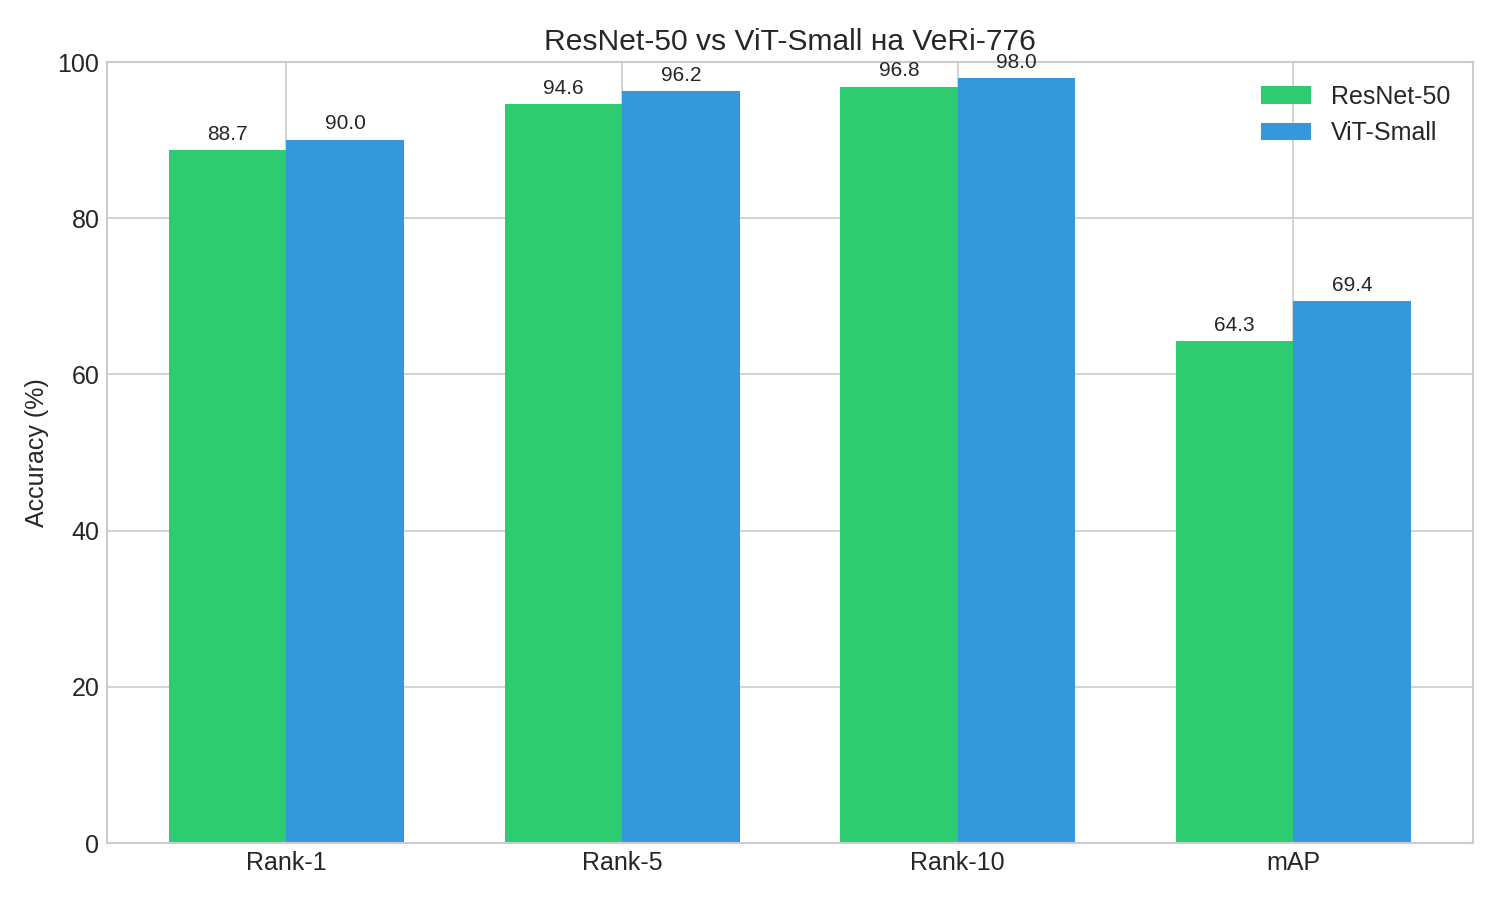
\includegraphics[width=0.85\textwidth]{images/comparison_metrics.png}
\caption{Сравнение метрик ResNet-50 и ViT-Small на VeRi-776}
\label{fig:comparison_metrics}
\end{figure}

\begin{figure}[H]
\centering
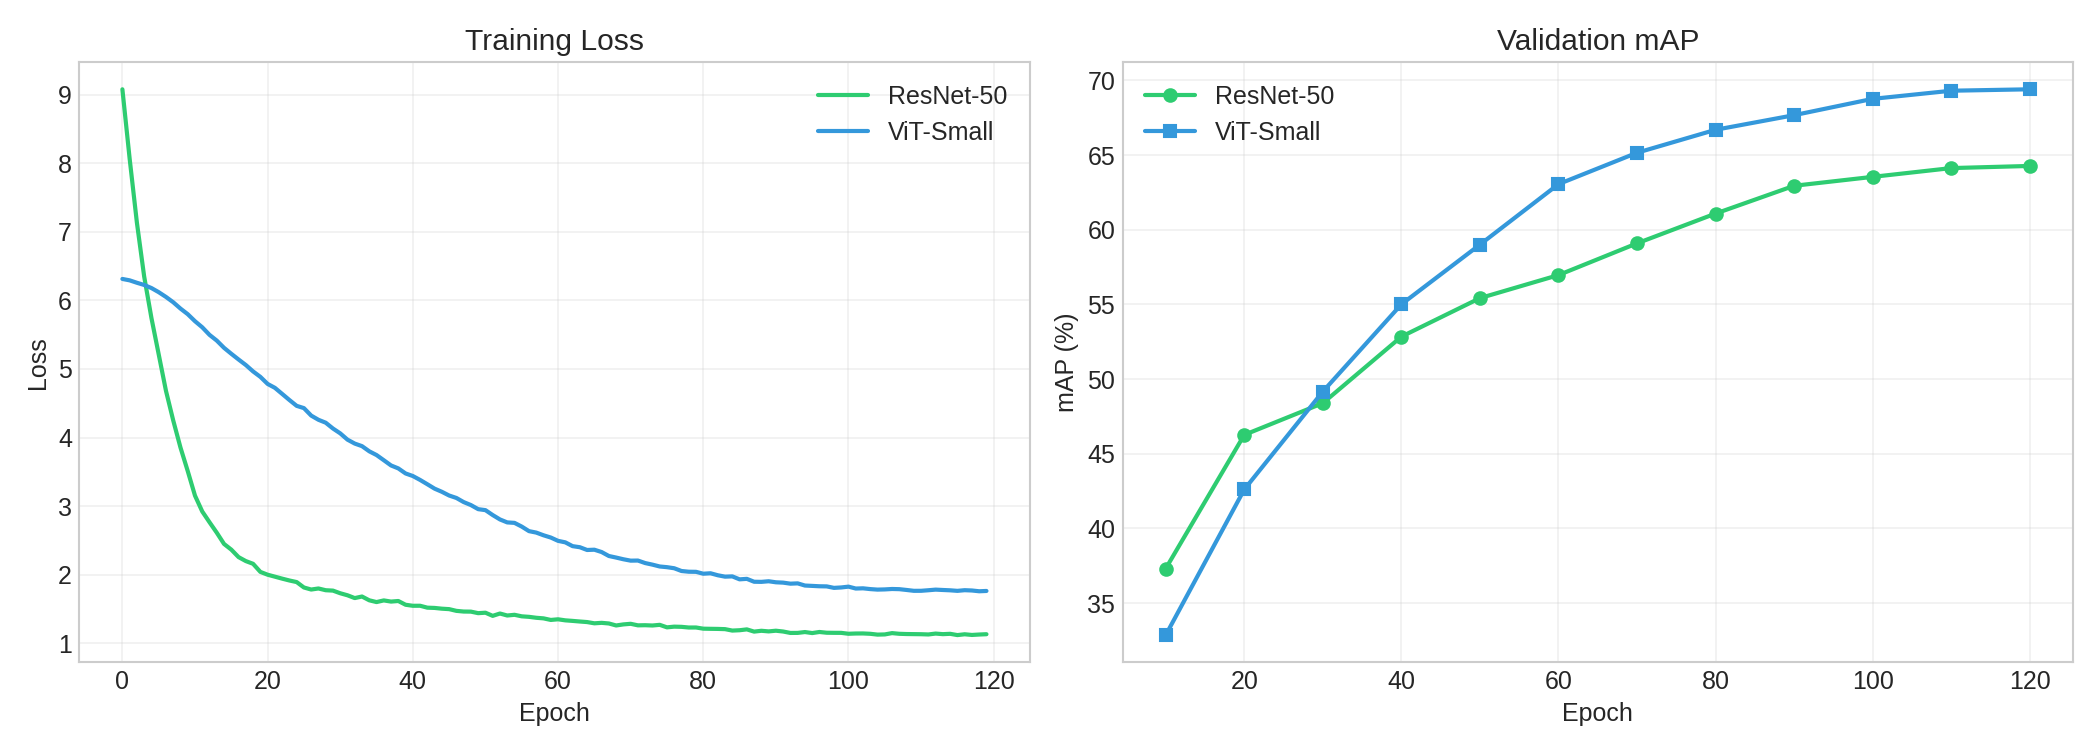
\includegraphics[width=0.85\textwidth]{images/training_curves_comparison.png}
\caption{Сравнение кривых обучения ResNet-50 и ViT-Small}
\label{fig:training_comparison}
\end{figure}

\subsection{Сравнение с существующими методами}

\begin{table}[H]
\centering
\small
\caption{Сравнение с State-of-the-Art на VeRi-776}
\label{tab:sota_comparison}
\begin{tabular}{l|c|c|l}
\hline
\textbf{Метод} & \textbf{Rank-1} & \textbf{mAP} & \textbf{Примечание} \\
\hline
OIFE (2018) & 68.3 & 48.0 & Orientation-aware \\
VAMI (2018) & 77.0 & 50.1 & Viewpoint-aware \\
PAMTRI (2020) & 92.9 & 71.8 & Multi-task \\
TransReID (2021) & 97.1 & 82.0 & ViT-Base + JPM \\
CLIP-ReID (2023) & 97.5 & 83.4 & CLIP pretrain \\
\hline
\textbf{ResNet-50 (наш)}  & 88.7 & 64.3 & Baseline CNN \\
\textbf{ResNet-101 (наш)} & 86.7 & 57.7 & Deeper CNN, хуже ResNet-50 \\
\textbf{ViT-Small (наш)}  & 90.0 & 69.4 & Baseline Transformer \\
\hline
\end{tabular}
\end{table}

\textbf{Анализ:} Наши baseline-результаты уступают SOTA методам, использующим:
\begin{itemize}
  \item Более крупные модели (ViT-Base, 86M параметров);
  \item Дополнительные модули (part-based, keypoints);
  \item Предобучение на больших данных (CLIP: 400M пар изображение-текст);
  \item Re-ranking и ensemble.
\end{itemize}
Ценность работы — в воспроизводимом сравнении CNN и Transformer на одинаковых условиях. Оценка показывает, что разрыв с SOTA (~13\% по mAP) обусловлен прежде всего размером backbone и качеством претрейна: замена ViT-Small на ViT-Base с ImageNet-21k инициализацией без изменения остальной архитектуры исторически сокращает этот разрыв до 5–7\% (TransReID, 2021), тогда как применение CLIP-претрейна полностью закрывает его за счёт семантического выравнивания визуальных и текстовых признаков.

\subsection{Визуализация результатов поиска}

Для демонстрации качественных результатов работы моделей приведены примеры поиска похожих транспортных средств. Каждая визуализация показывает query-изображение (запрос) слева и топ-5 наиболее похожих результатов из gallery. Зелёная рамка указывает на правильно найденное транспортное средство (совпадает ID с query), красная — на ошибочно найденное.

\subsubsection{Успешные примеры работы ViT-Small}

\begin{figure}[H]
\centering
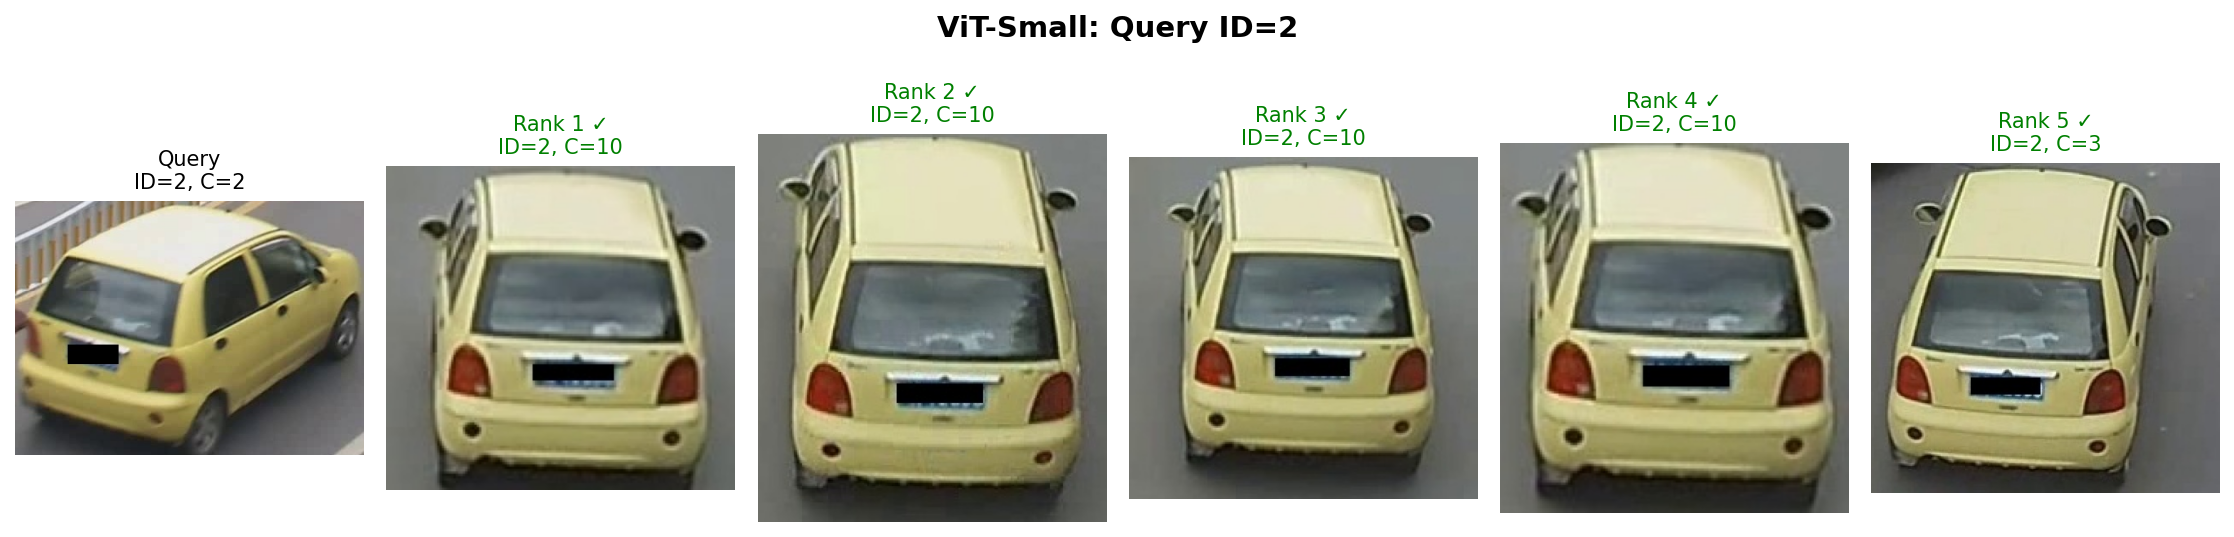
\includegraphics[width=\textwidth]{images/vit_example_1.png}
\caption{Идеальный результат ViT-Small на запросе ID=2 (жёлтый хэтчбек): все 5 результатов правильны. Модель успешно находит тот же автомобиль с разных ракурсов и при различном освещении, демонстрируя устойчивость механизма self-attention к изменениям условий съёмки}
\label{fig:vit_example_1}
\end{figure}

\begin{figure}[H]
\centering
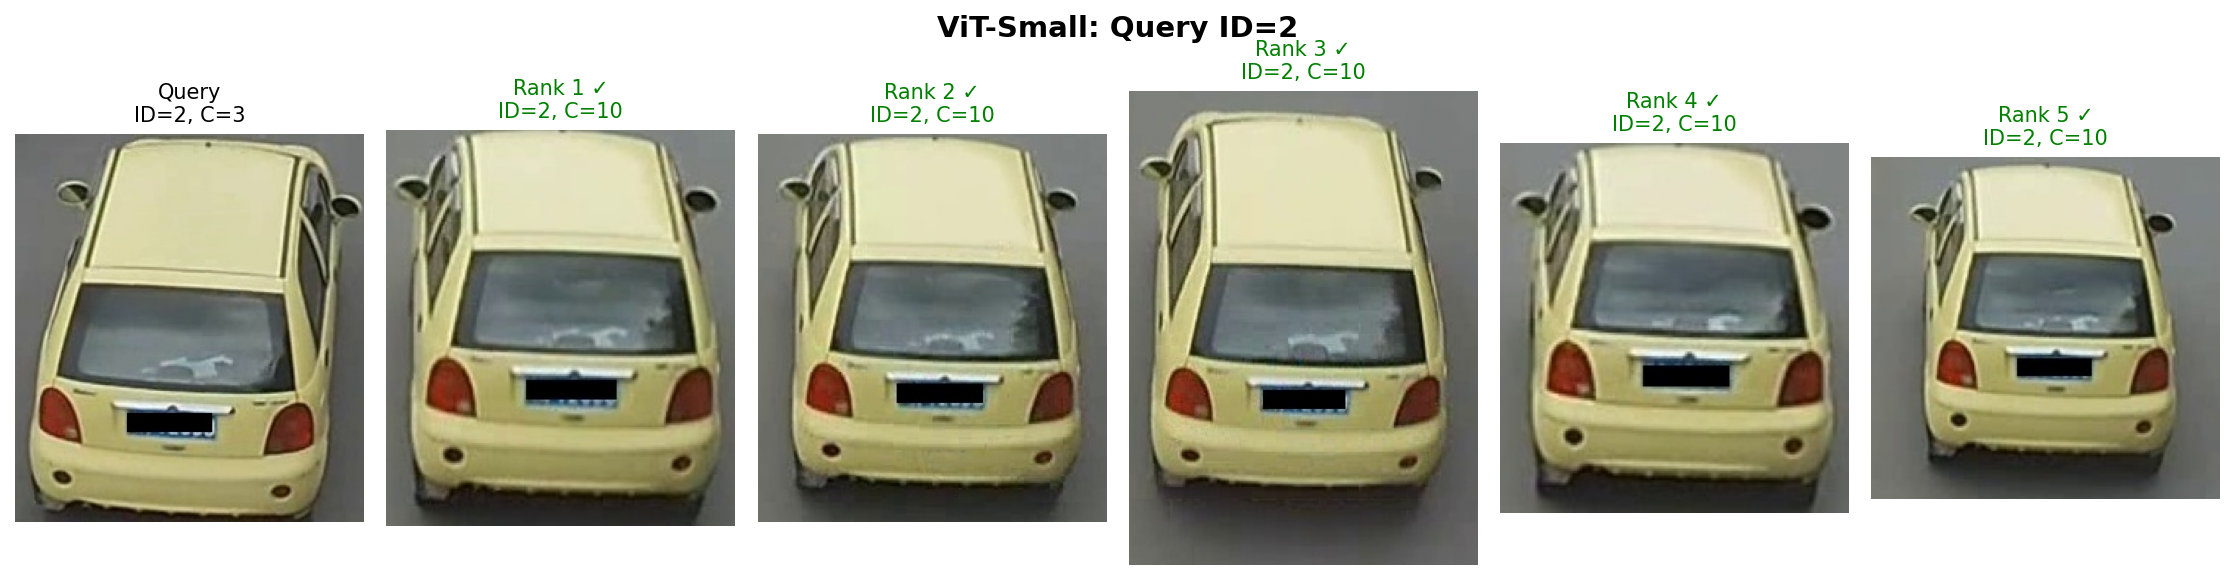
\includegraphics[width=\textwidth]{images/vit_example_2.png}
\caption{ViT-Small на запросе ID=2 с другого ракурса: снова идеальный результат (5/5). Модель корректно идентифицирует транспортное средство даже при значительном изменении угла обзора, что подтверждает способность трансформера улавливать глобальные инвариантные признаки}
\label{fig:vit_example_2}
\end{figure}

\begin{figure}[H]
\centering
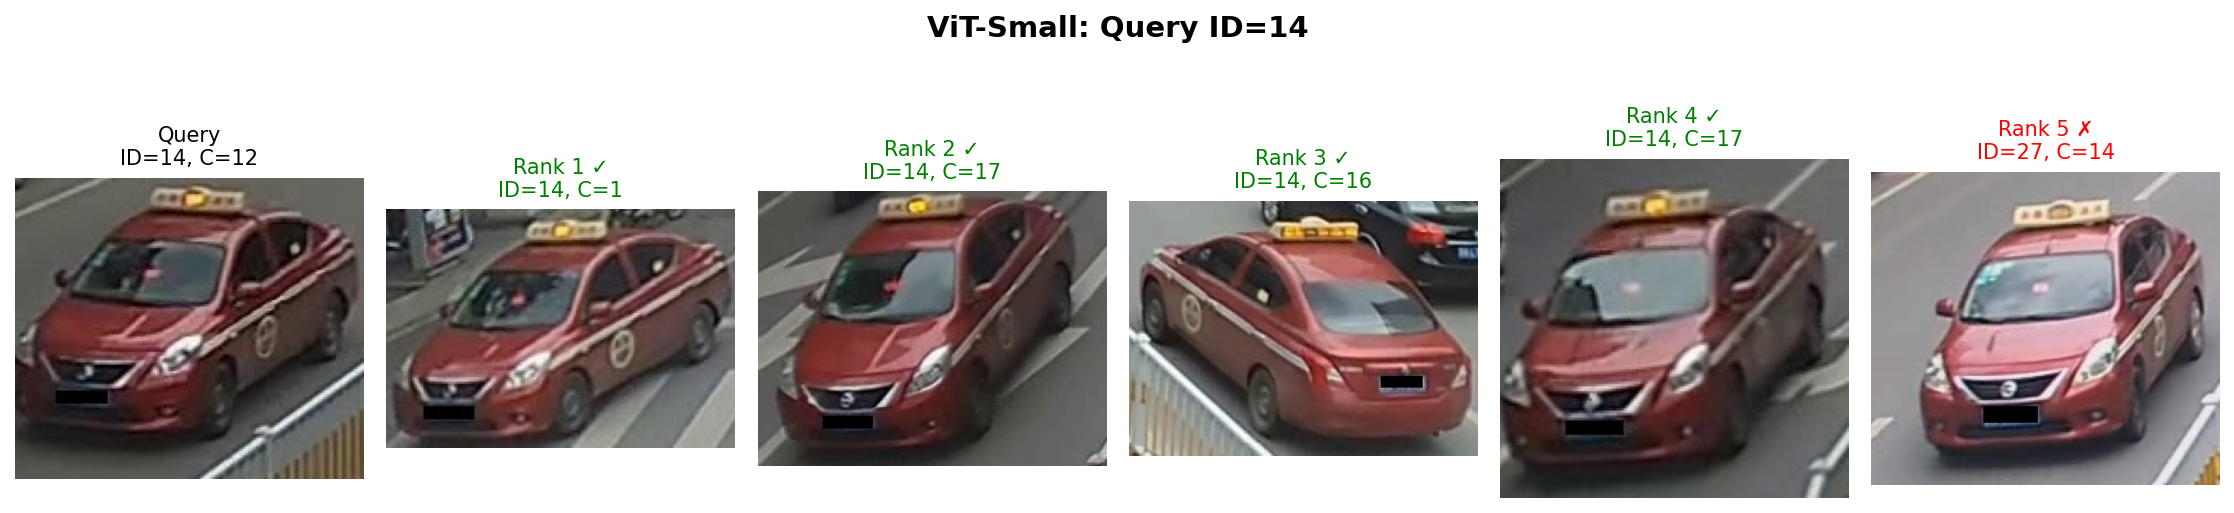
\includegraphics[width=\textwidth]{images/vit_example_3.png}
\caption{ViT-Small на запросе ID=14 (красный минивэн): 4 из 5 результатов правильны. Модель допускает единичные ошибки при наличии схожих транспортных средств того же цвета, но в целом показывает хорошую различительную способность}
\label{fig:vit_example_3}
\end{figure}

\subsubsection{Сложные случаи для ViT-Small}

\begin{figure}[H]
\centering
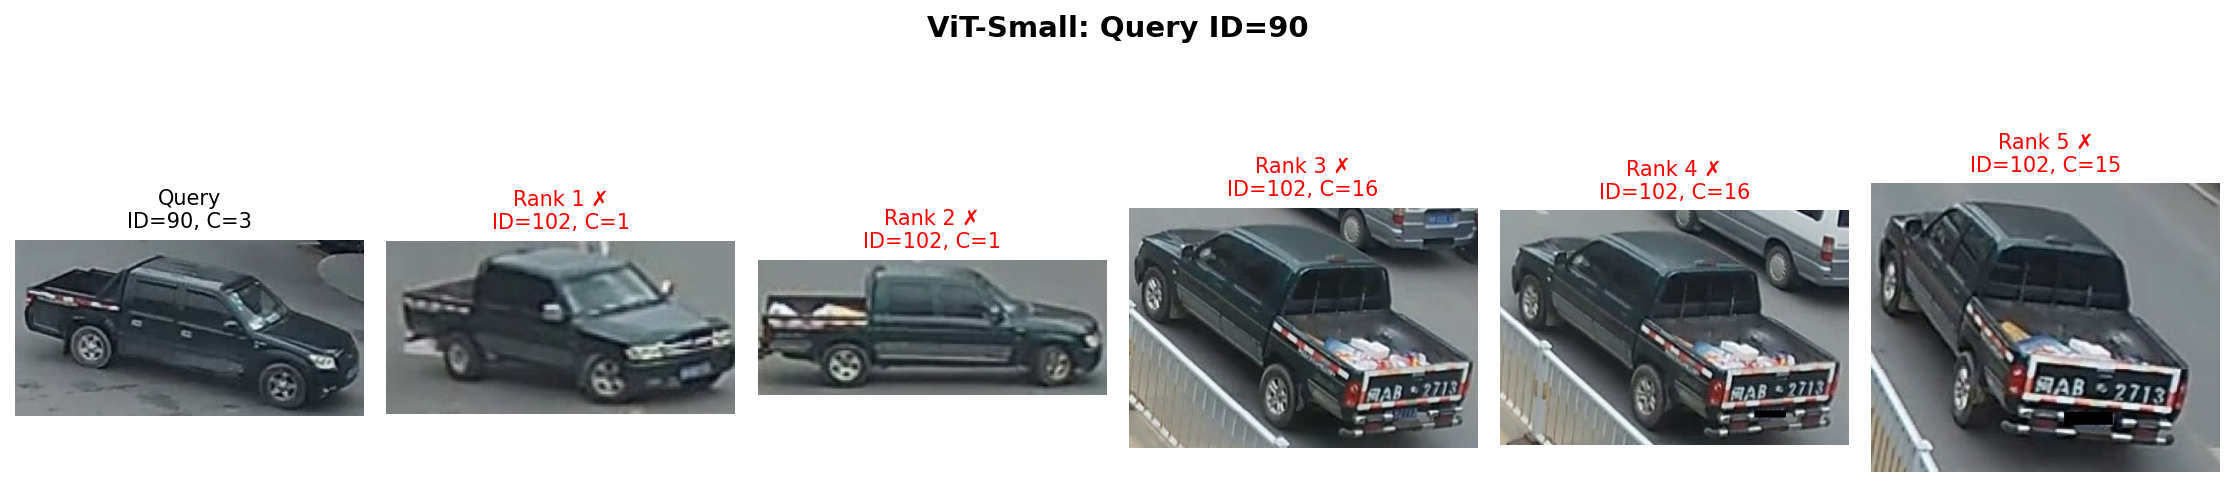
\includegraphics[width=\textwidth]{images/vit_example_5.png}
\caption{Провал ViT-Small на запросе ID=90 (чёрный внедорожник): все топ-5 результатов ошибочны. Модель испытывает трудности с тёмными транспортными средствами — низкая контрастность затрудняет выделение различительных признаков, что приводит к смешению схожих по форме автомобилей}
\label{fig:vit_example_5}
\end{figure}

\subsubsection{Успешные примеры работы ResNet-50}

\begin{figure}[H]
\centering
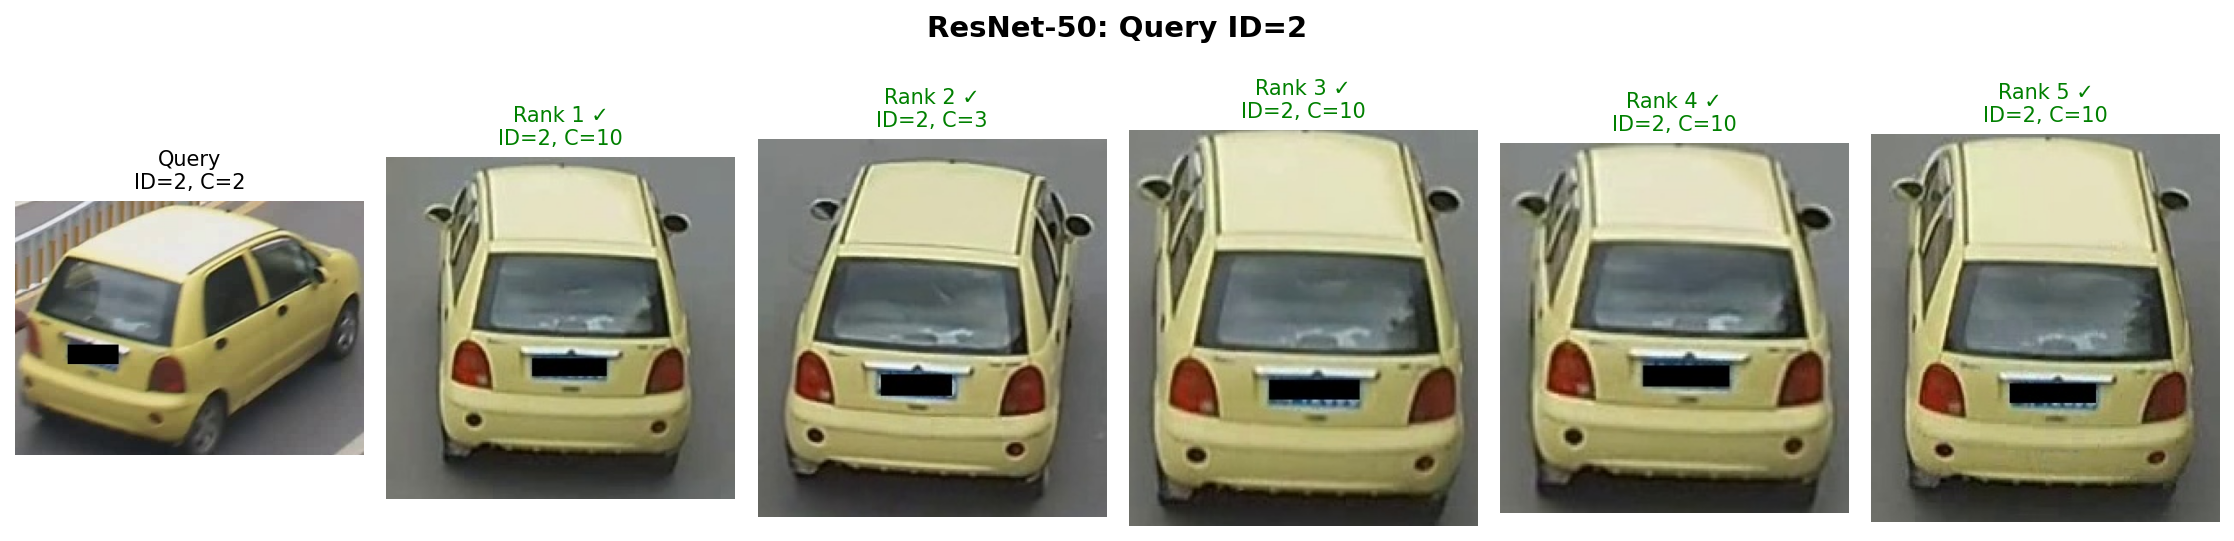
\includegraphics[width=\textwidth]{images/resnet50_example_1.png}
\caption{Идеальный результат ResNet-50 на запросе ID=2 (жёлтый хэтчбек): все 5 результатов правильны. CNN-модель эффективно использует локальные признаки (детали кузова, цвет, форма задней части) для точной идентификации}
\label{fig:resnet_example_1}
\end{figure}

\begin{figure}[H]
\centering
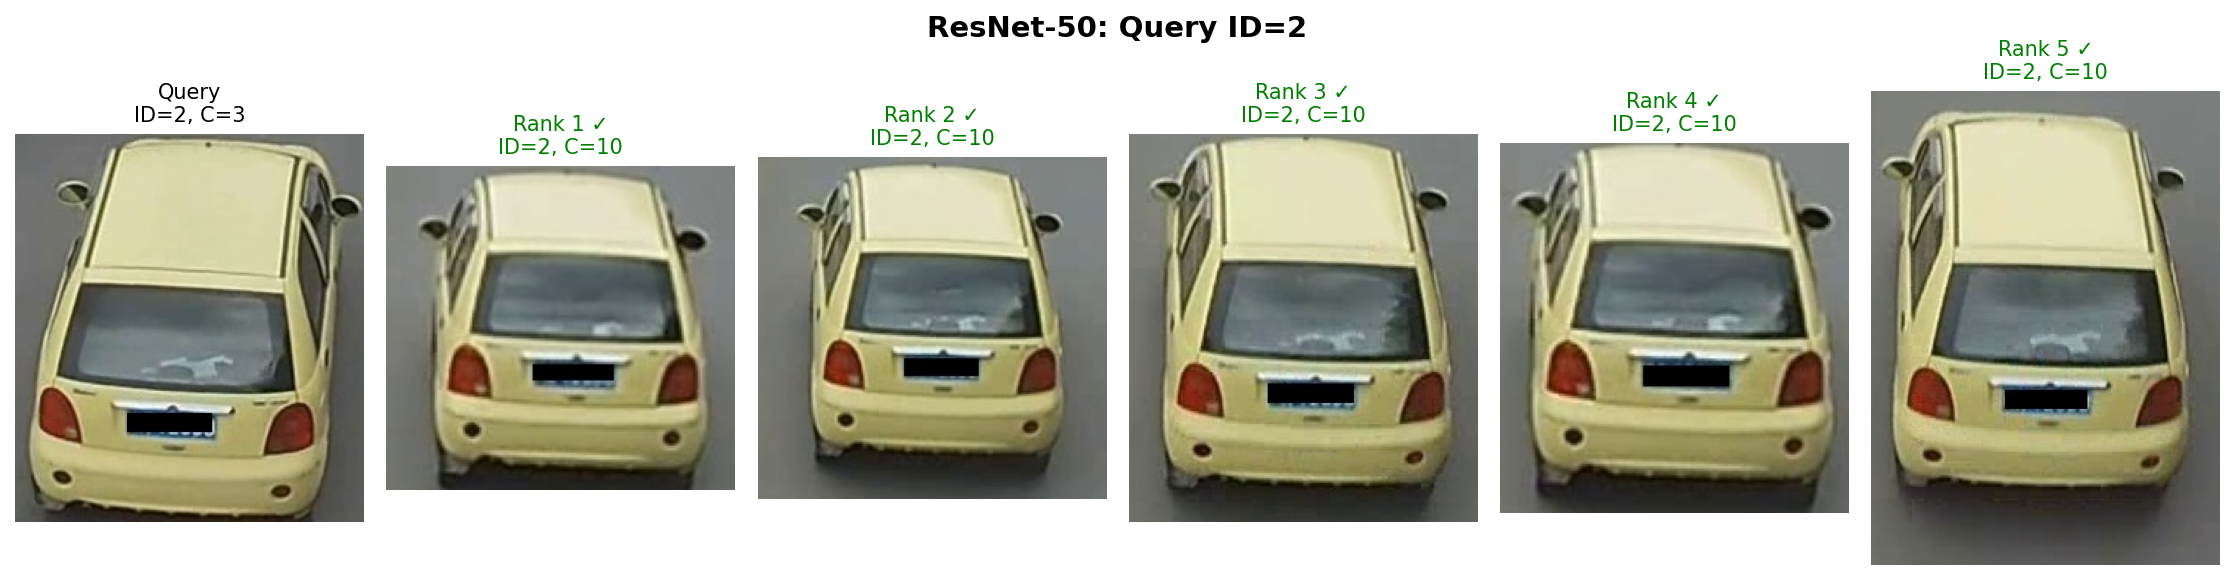
\includegraphics[width=\textwidth]{images/resnet50_example_2.png}
\caption{ResNet-50 на запросе ID=2 с другого ракурса: снова идеальный результат (5/5). Модель демонстрирует робастность свёрточных признаков к изменению точки обзора, успешно сопоставляя локальные паттерны}
\label{fig:resnet_example_2}
\end{figure}

\begin{figure}[H]
\centering
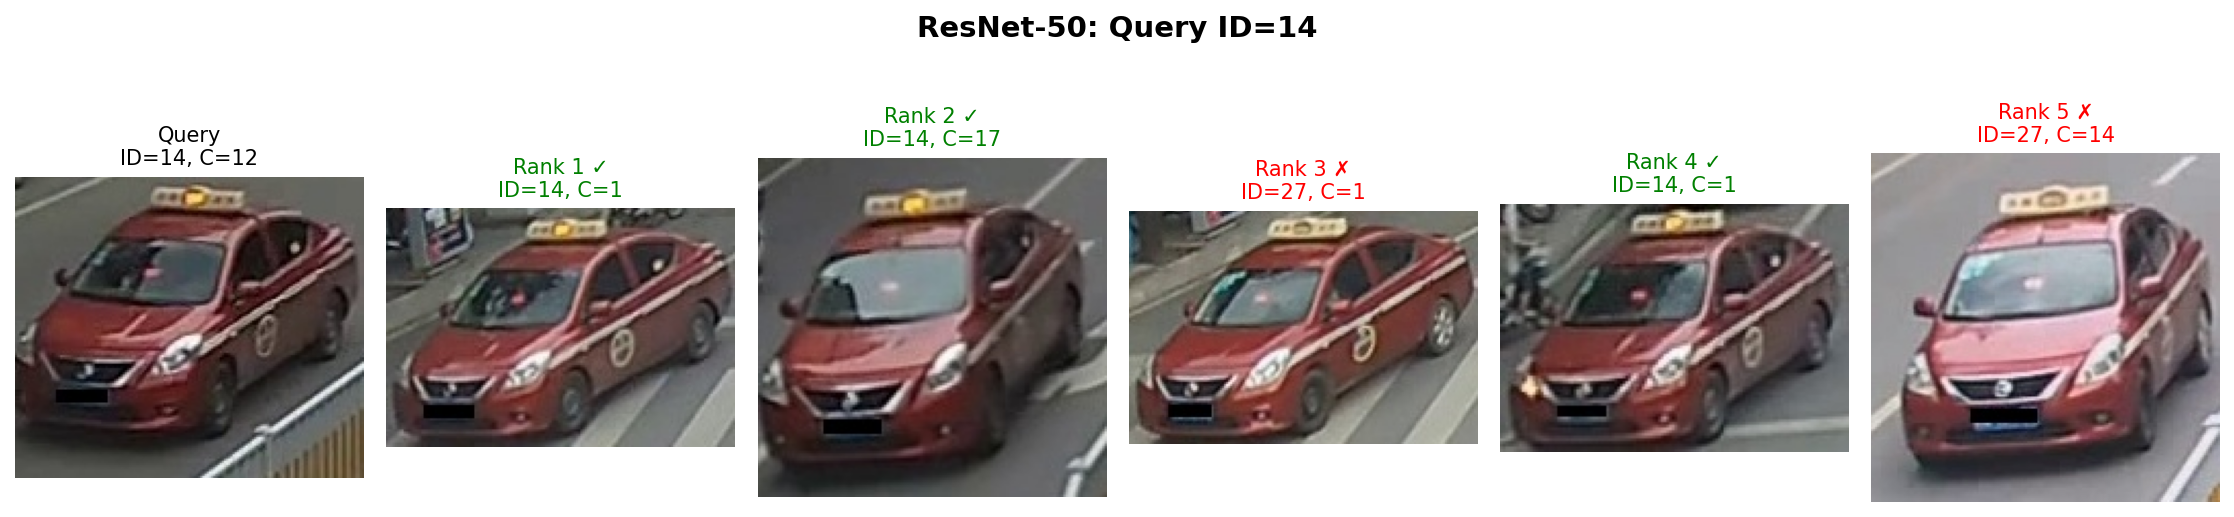
\includegraphics[width=\textwidth]{images/resnet50_example_3.png}
\caption{ResNet-50 на запросе ID=14 (красный минивэн): 3 из 5 результатов правильны. Модель справляется с задачей, но уступает ViT-Small на том же запросе, что указывает на ограничения локальных свёрточных признаков при различении похожих транспортных средств}
\label{fig:resnet_example_3}
\end{figure}

\subsubsection{Сложные случаи для ResNet-50}

\begin{figure}[H]
\centering
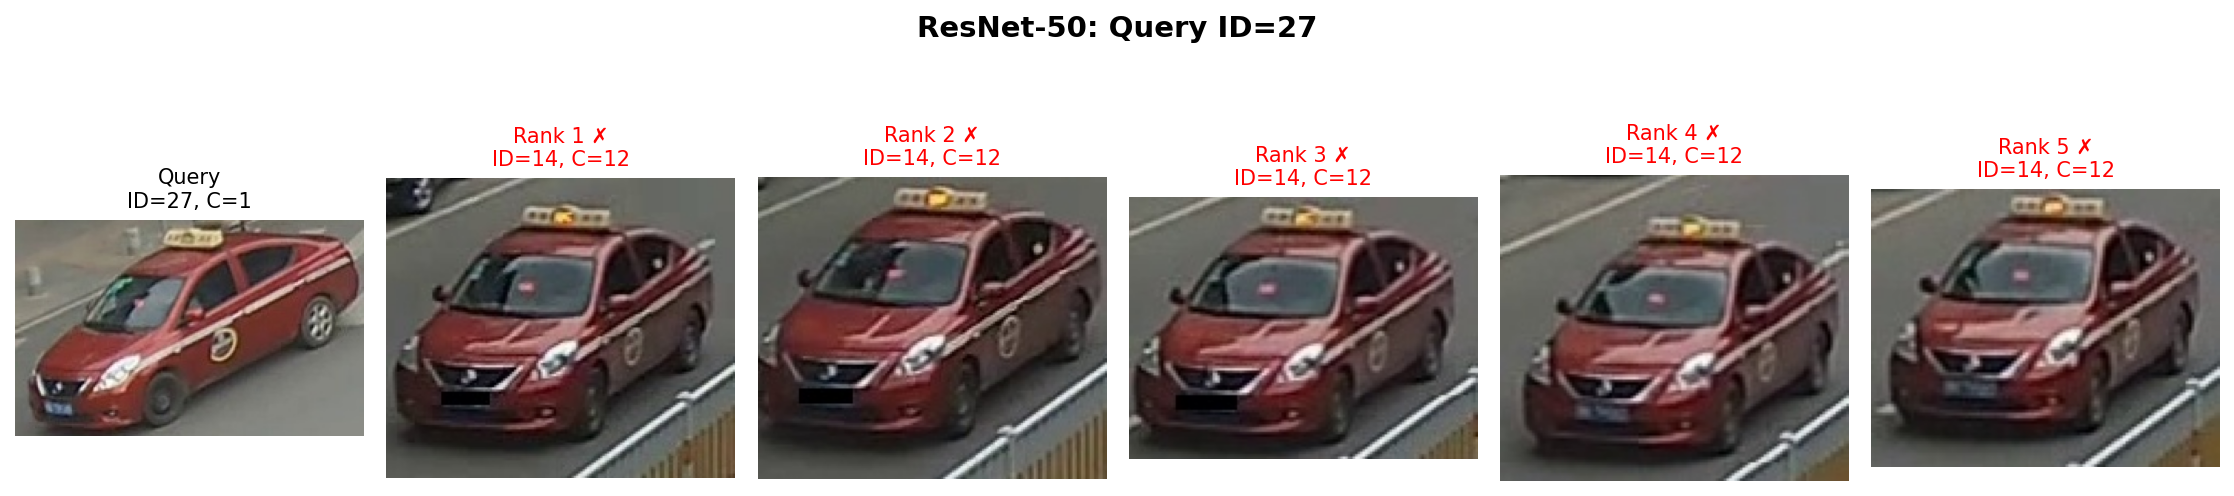
\includegraphics[width=\textwidth]{images/resnet50_example_4.png}
\caption{Провал ResNet-50 на запросе ID=27 (темно-красный седан): все топ-5 результатов ошибочны. Ограниченное рецептивное поле CNN затрудняет различение транспортных средств схожей формы и цвета — модель фокусируется на локальных паттернах, упуская глобальный контекст}
\label{fig:resnet_example_4}
\end{figure}

\subsubsection{Прямое сравнение моделей}

\begin{figure}[H]
\centering
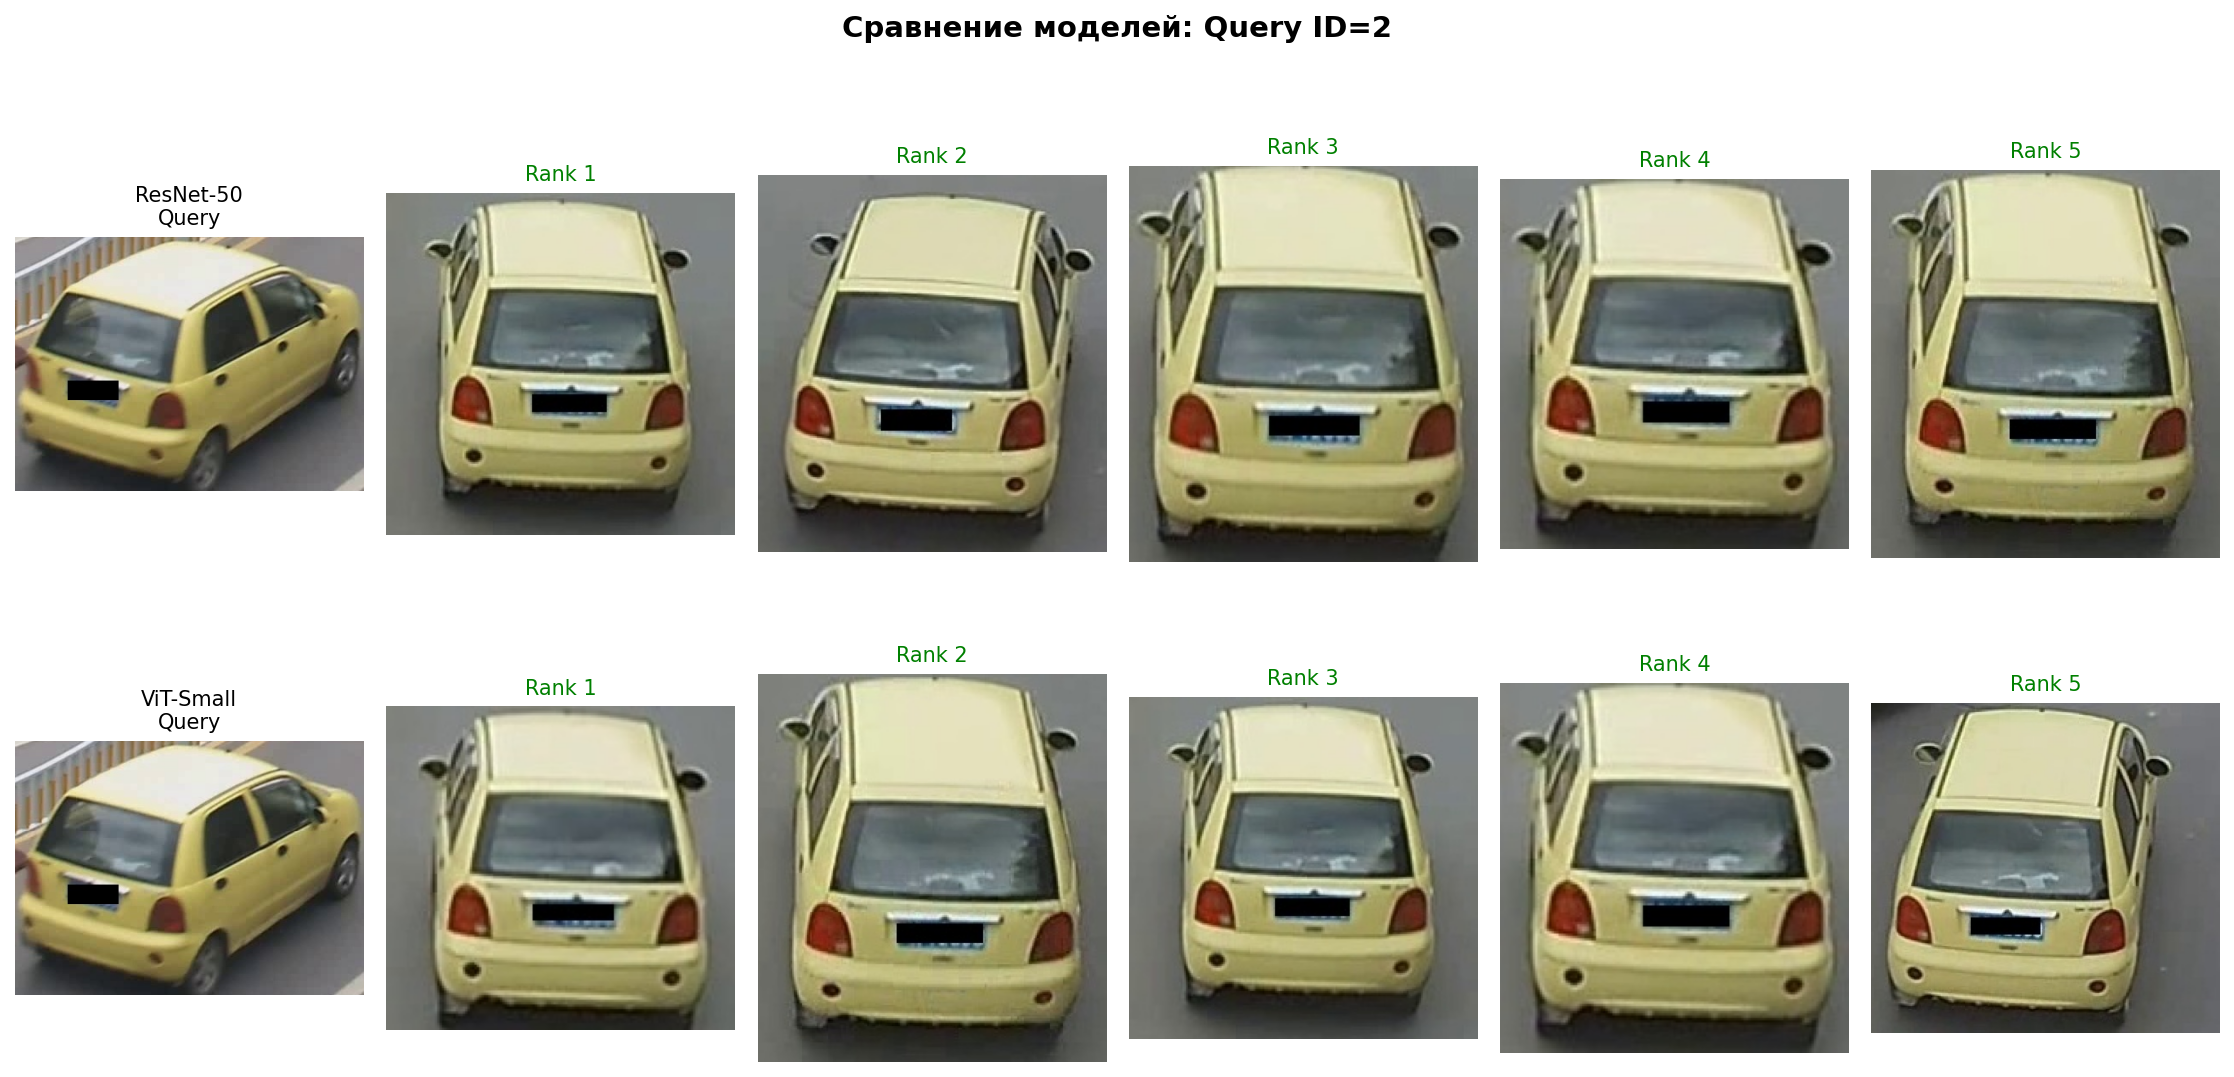
\includegraphics[width=\textwidth]{images/comparison_query_0.png}
\caption{Сравнение на запросе ID=2 (жёлтый хэтчбек): обе модели показывают идеальный результат (5/5). ResNet-50 (вверху) и ViT-Small (внизу) одинаково эффективны на «простых» запросах с уникальными цветовыми и формовыми признаками}
\label{fig:comparison_0}
\end{figure}

\begin{figure}[H]
\centering
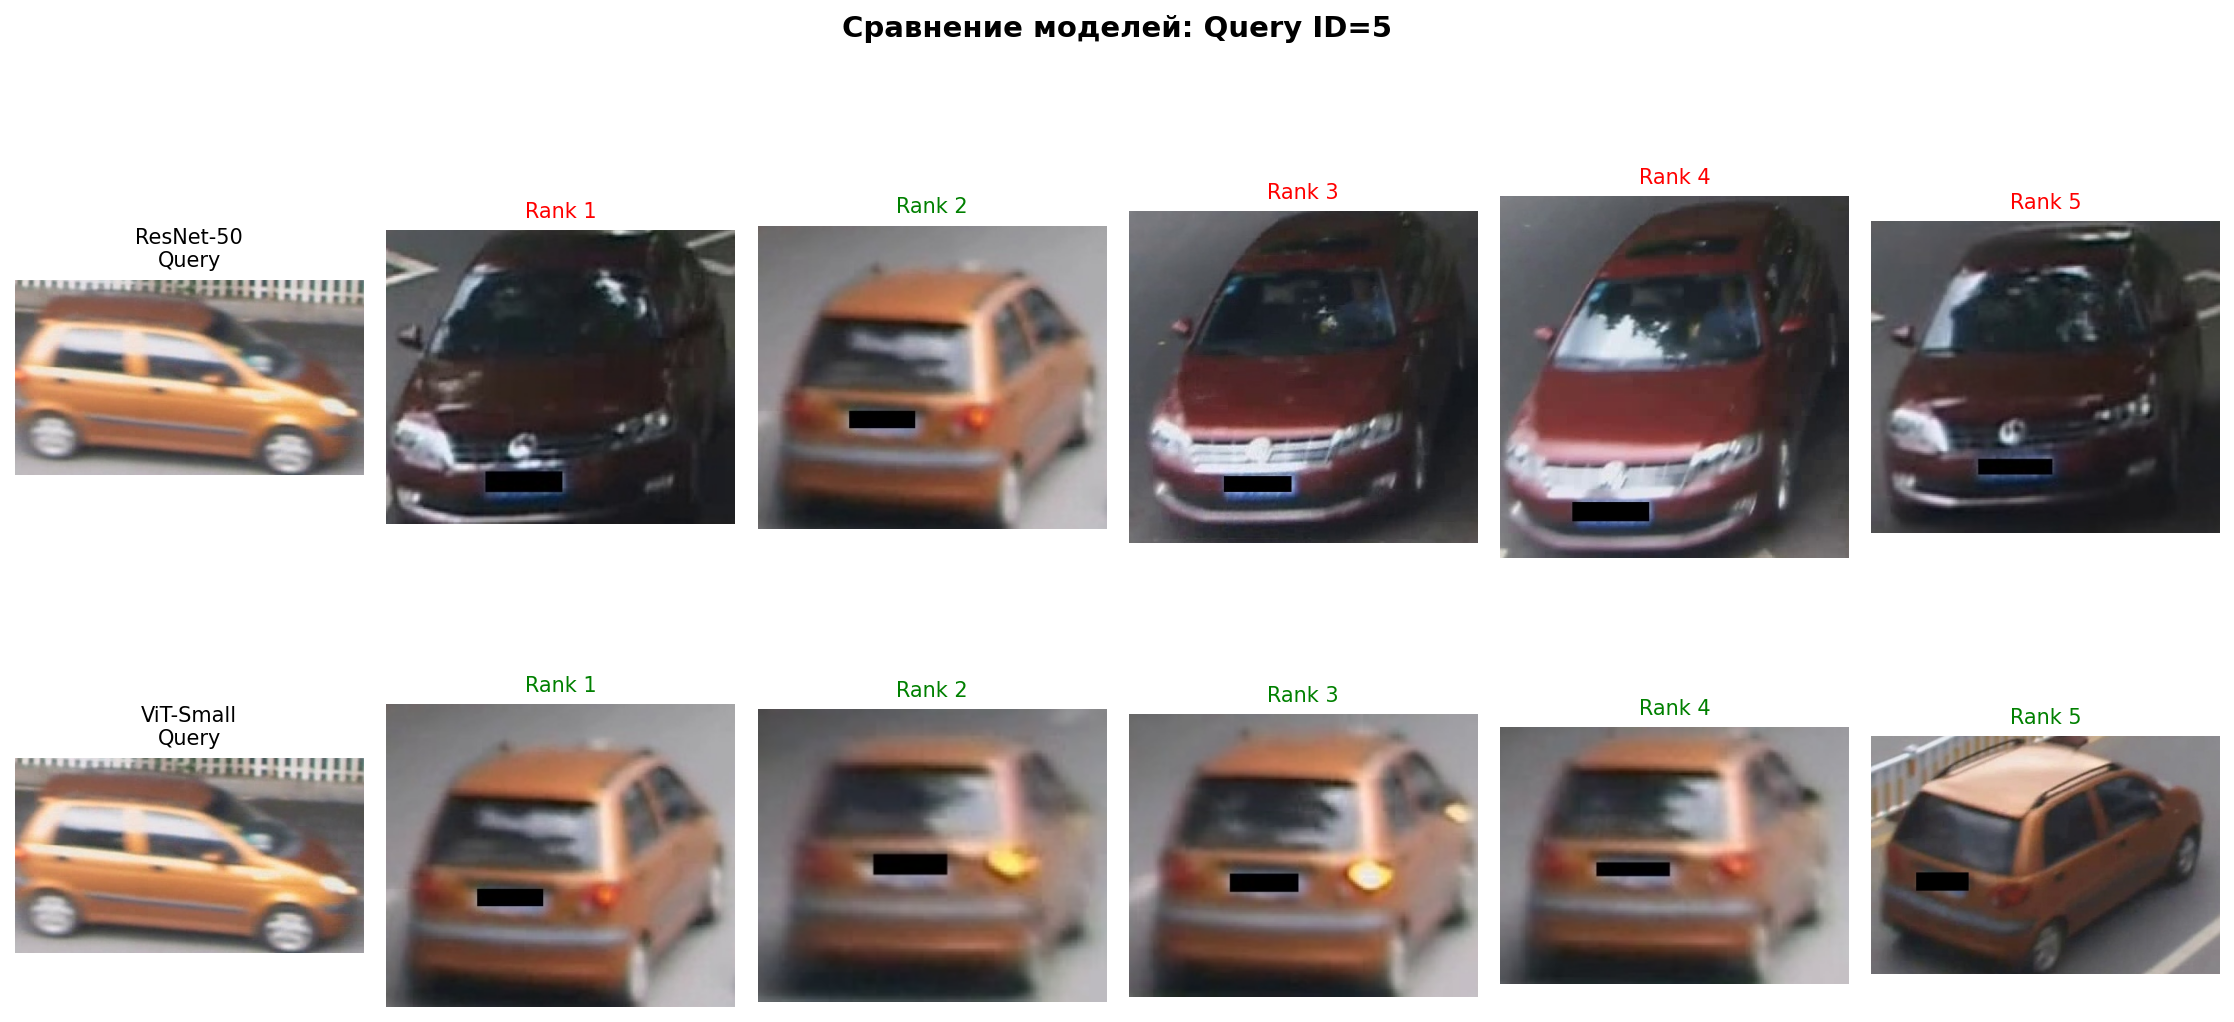
\includegraphics[width=\textwidth]{images/comparison_query_15.png}
\caption{Сравнение на запросе ID=5 (оранжевый хэтчбек): ViT-Small побеждает. ViT (внизу) находит 4 правильных результата благодаря глобальному вниманию, в то время как ResNet-50 (вверху) допускает больше ошибок из-за ограниченного рецептивного поля}
\label{fig:comparison_15}
\end{figure}

\begin{figure}[H]
\centering
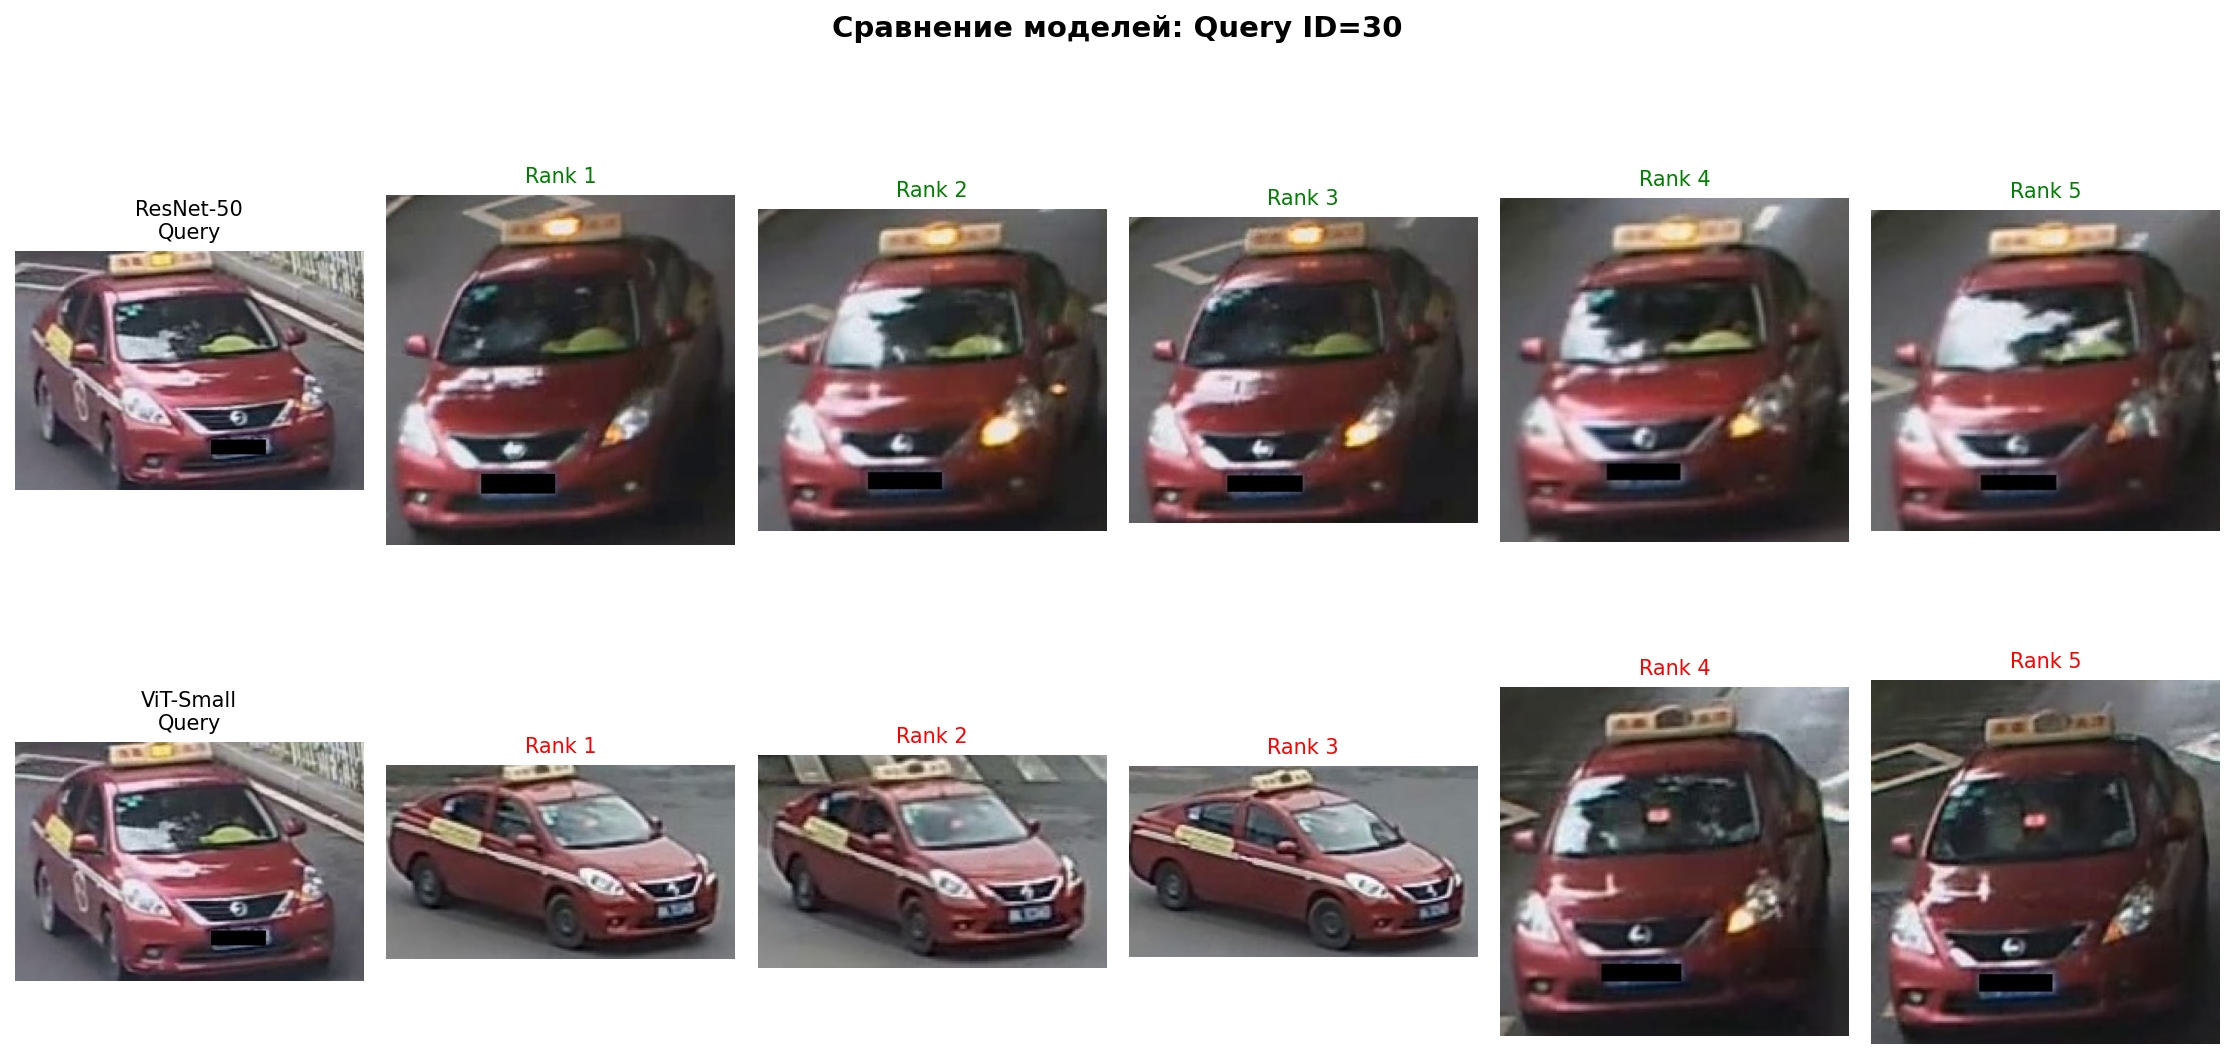
\includegraphics[width=\textwidth]{images/comparison_query_51.png}
\caption{Сравнение на запросе ID=30 (темно-красный седан): ResNet-50 побеждает. ResNet (вверху) показывает идеальный результат (5/5), используя локальные детали кузова, в то время как ViT-Small (внизу) допускает ошибки (3/5) на этом конкретном запросе}
\label{fig:comparison_51}
\end{figure}

\begin{figure}[H]
\centering
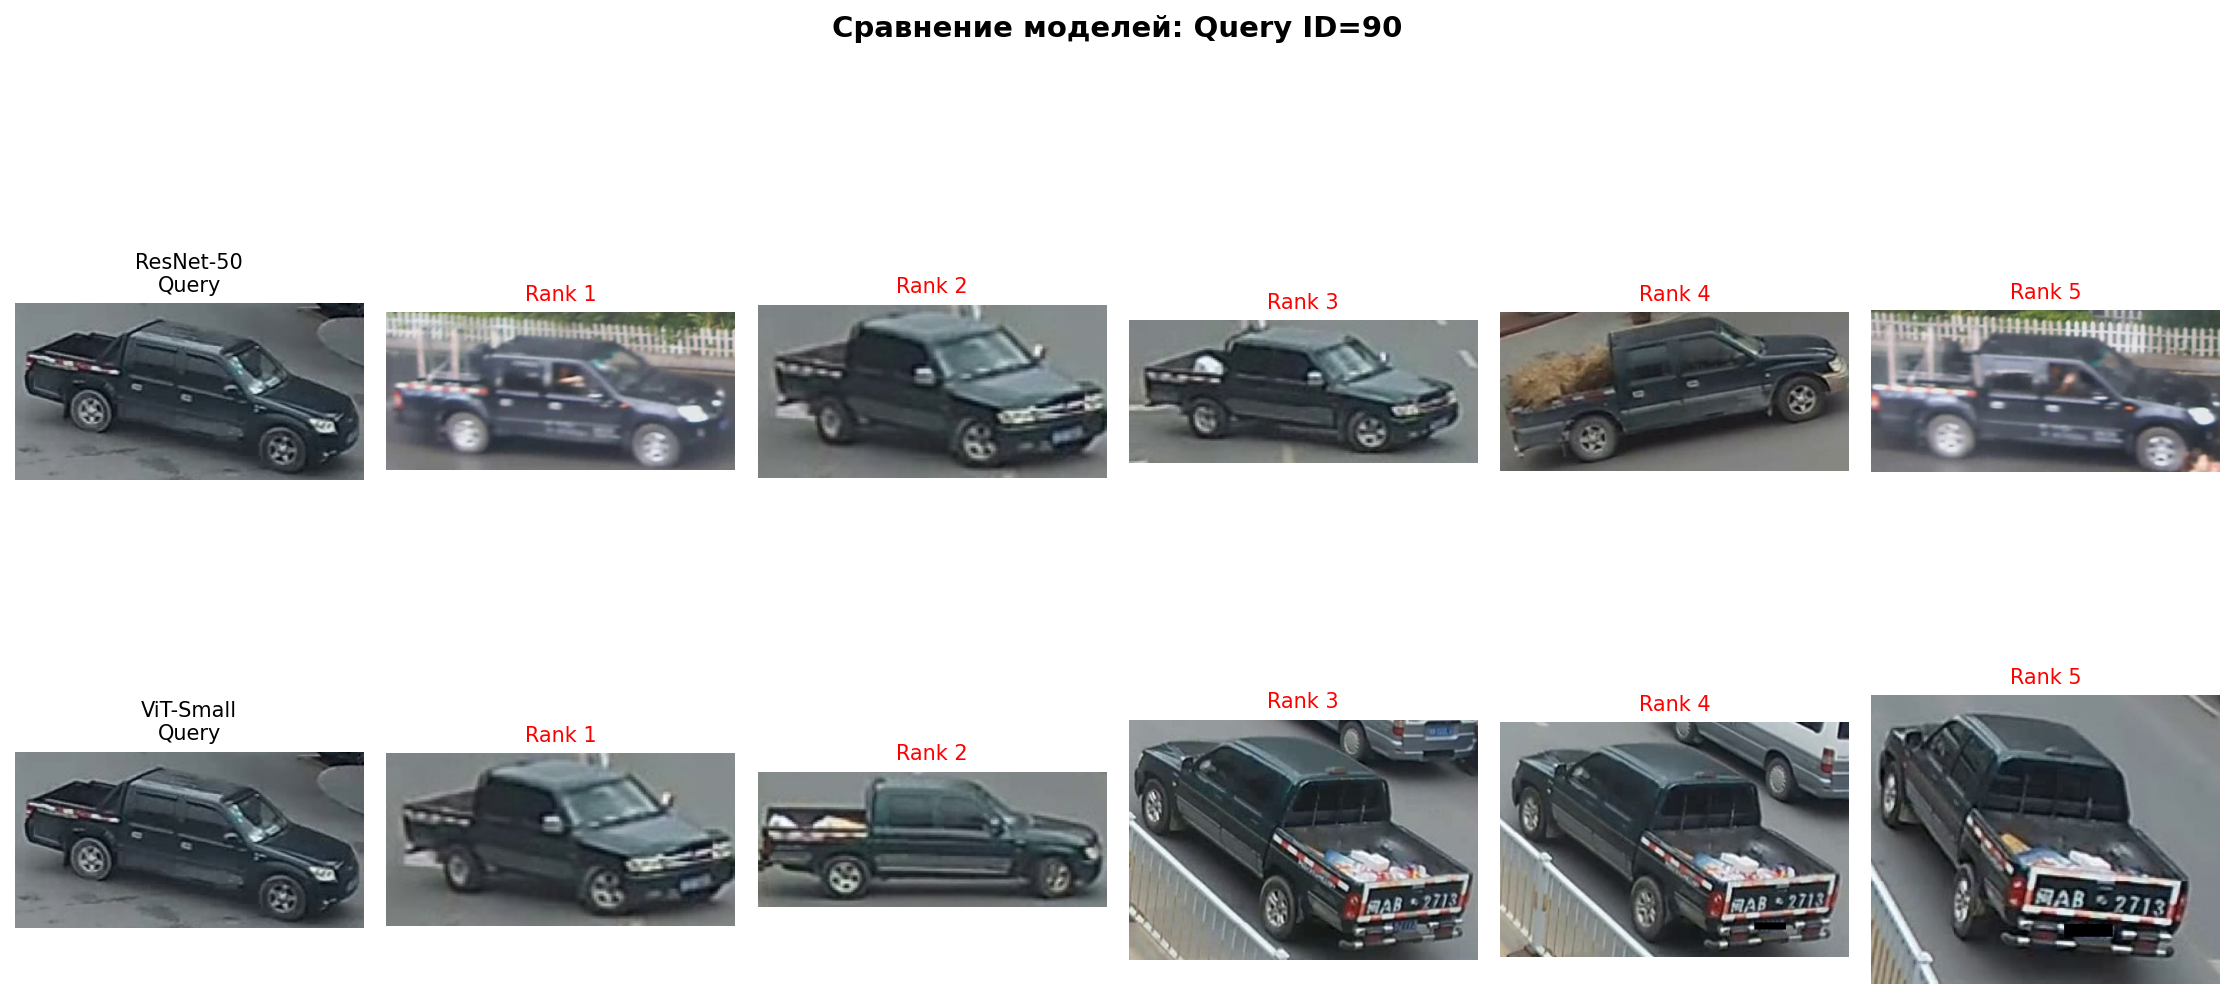
\includegraphics[width=\textwidth]{images/comparison_query_133.png}
\caption{Сравнение на запросе ID=90 (чёрный внедорожник): обе модели терпят неудачу (0/5). Этот пример иллюстрирует общую проблему — низкая контрастность и схожая форма затрудняют идентификацию для обеих архитектур, указывая на необходимость дополнительных техник (re-ranking, attention to parts)}
\label{fig:comparison_133}
\end{figure}

\textbf{Качественный анализ:}
\begin{itemize}
  \item Обе модели показывают отличные результаты на запросах с уникальными признаками (яркий цвет, характерная форма), достигая идеальной точности 5/5 в топ-5;
  \item ViT-Small демонстрирует преимущество на сложных запросах благодаря механизму self-attention, учитывающему глобальный контекст изображения;
  \item ResNet-50 эффективен при наличии чётких локальных признаков, но испытывает трудности при различении транспортных средств со схожей текстурой и формой;
  \item Оба подхода испытывают серьёзные проблемы с тёмными транспортными средствами (низкая контрастность) — требуется улучшение предобработки или дополнительные модули внимания;
  \item Приведённые примеры объясняют разницу в метриках (ViT: 90.0\% Rank-1 vs ResNet: 88.7\%) и демонстрируют, что в большинстве случаев обе модели работают хорошо, но на «пограничных» сложных запросах ViT показывает лучшую робастность.
\end{itemize}

\section{Анализ маршрутов транспортных средств по камерам}
\label{sec:camera_analysis}

Датасет VeRi-776 содержит 20 камер, расположенных в реальной дорожной сети. Анализ
траекторий транспортных средств позволяет понять структуру наблюдений и сложность
задачи повторной идентификации в зависимости от удалённости камер.

\subsection{Граф переходов между камерами}

По обучающей выборке (37\,778 изображений, 575 транспортных средств) построен направленный
граф: вершина~--- камера, ребро $\mathrm{C}_i \to \mathrm{C}_j$ означает, что
транспортное средство зафиксировано сначала камерой~$i$, затем камерой~$j$.
Вес вершины пропорционален числу уникальных ТС через неё, вес ребра~---
числу таких переходов.

\begin{figure}[H]
  \centering
  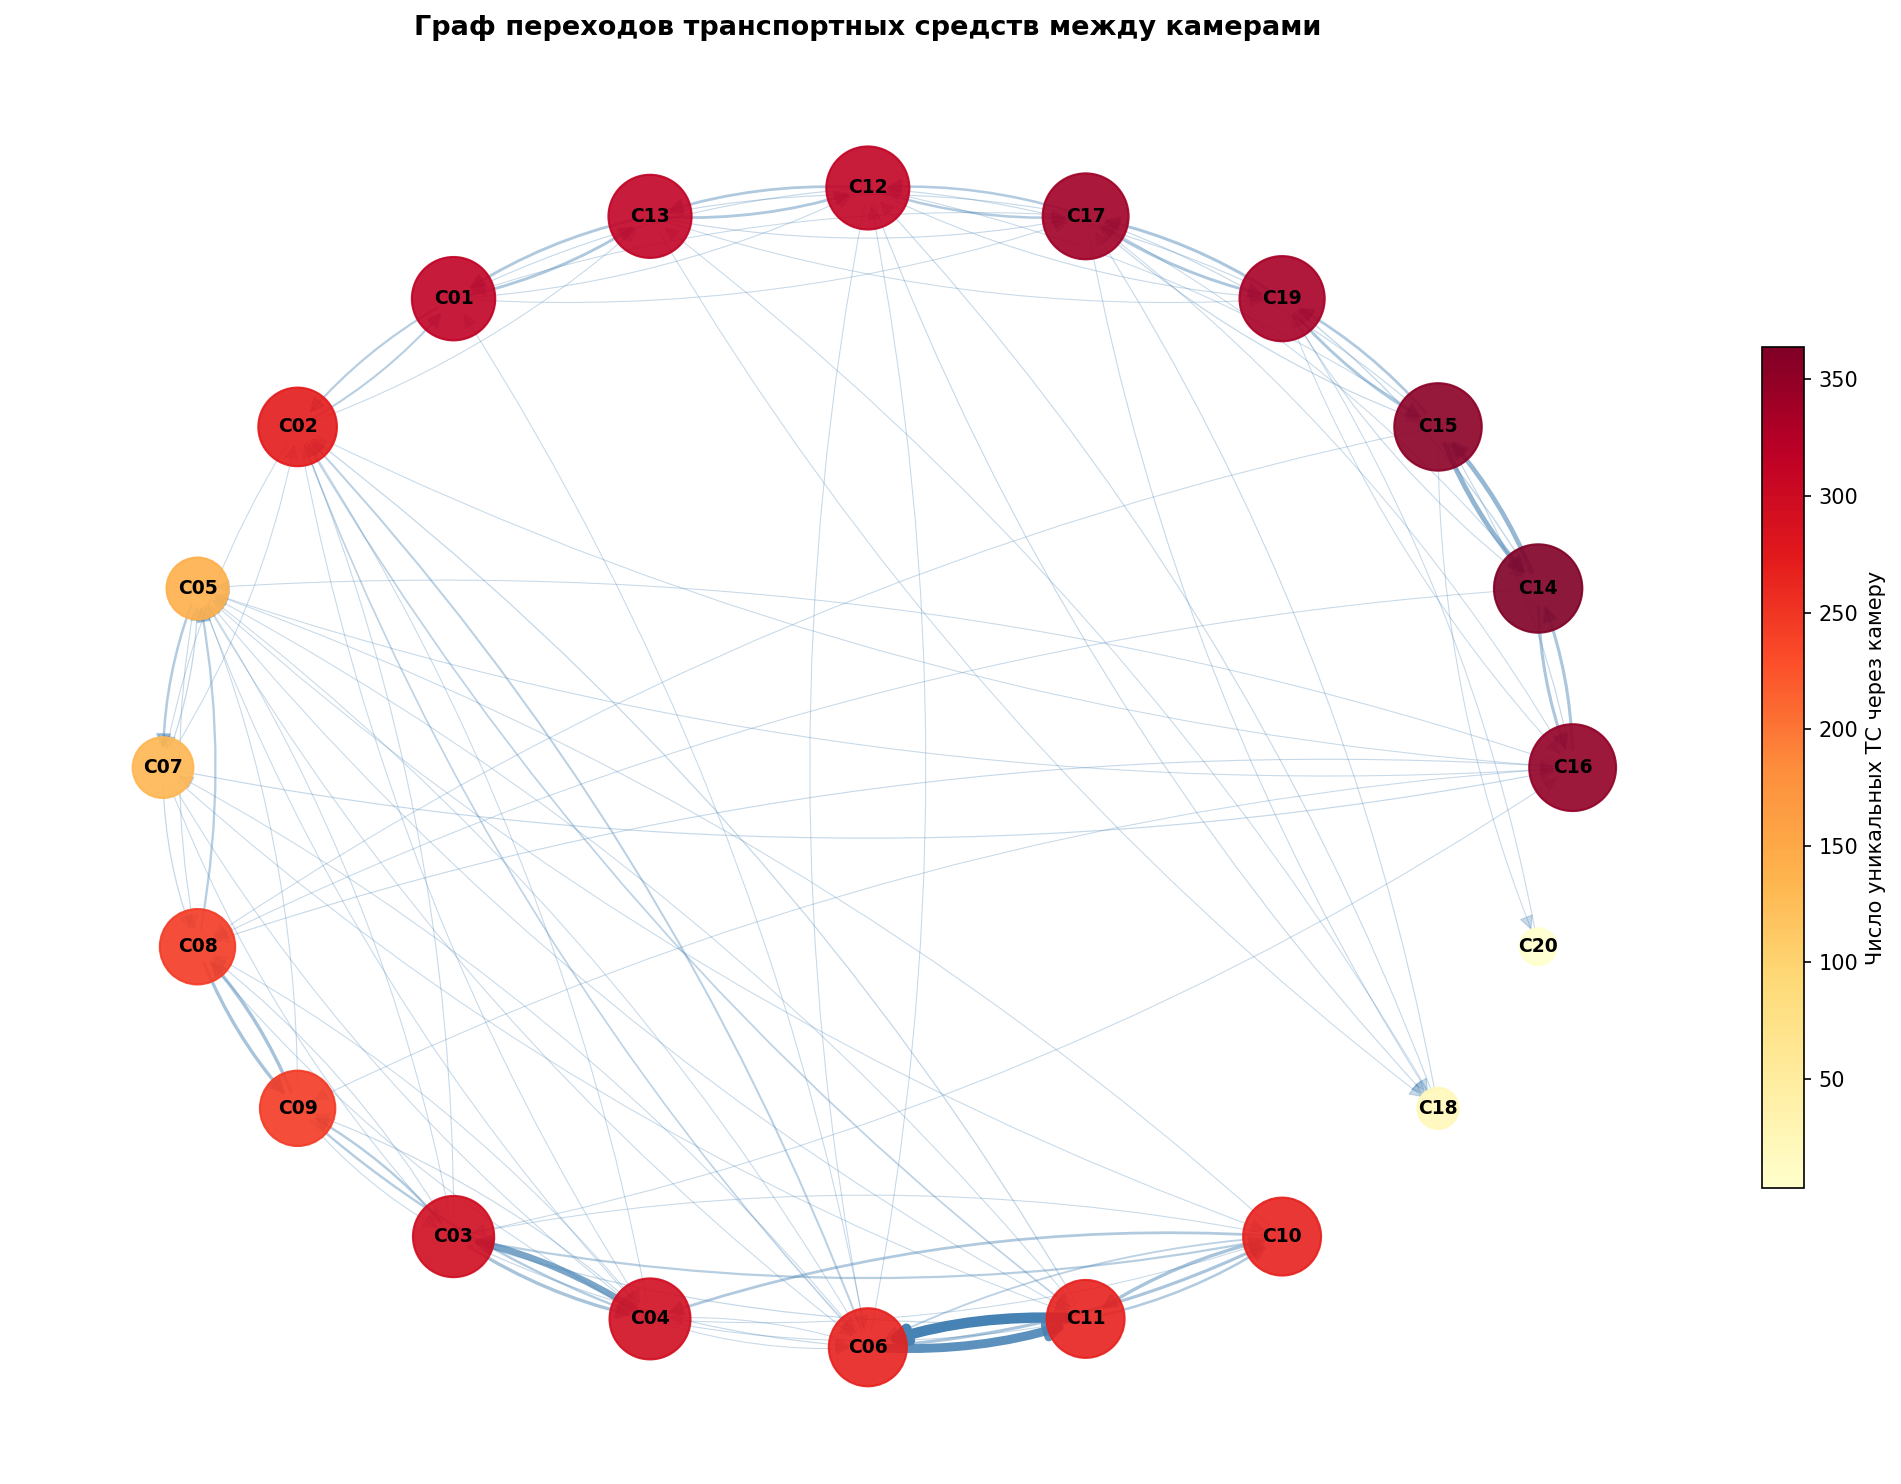
\includegraphics[width=0.85\textwidth]{images/camera_route_graph.png}
  \caption{Граф переходов транспортных средств между камерами VeRi-776.
    Размер вершины пропорционален числу ТС, толщина ребра~--- частоте
    перехода. Стрелки показывают направление движения.}
  \label{fig:camera_route_graph}
\end{figure}

Основные характеристики графа:

\begin{itemize}
  \item Граф содержит 20 вершин и 108 направленных рёбер (из 380 возможных),
    что свидетельствует о выраженной топологии дорожной сети;
  \item Камеры C11 и C06 образуют наиболее нагруженное двунаправленное ребро
    (990 и 825 переходов соответственно) — по всей видимости, они расположены
    на одном перекрёстке или прямом участке трассы;
  \item Среднее число камер на маршруте одного ТС: \textbf{8.9} (от 2 до 18),
    что подтверждает протяжённость наблюдаемых траекторий.
\end{itemize}

\begin{figure}[H]
  \centering
  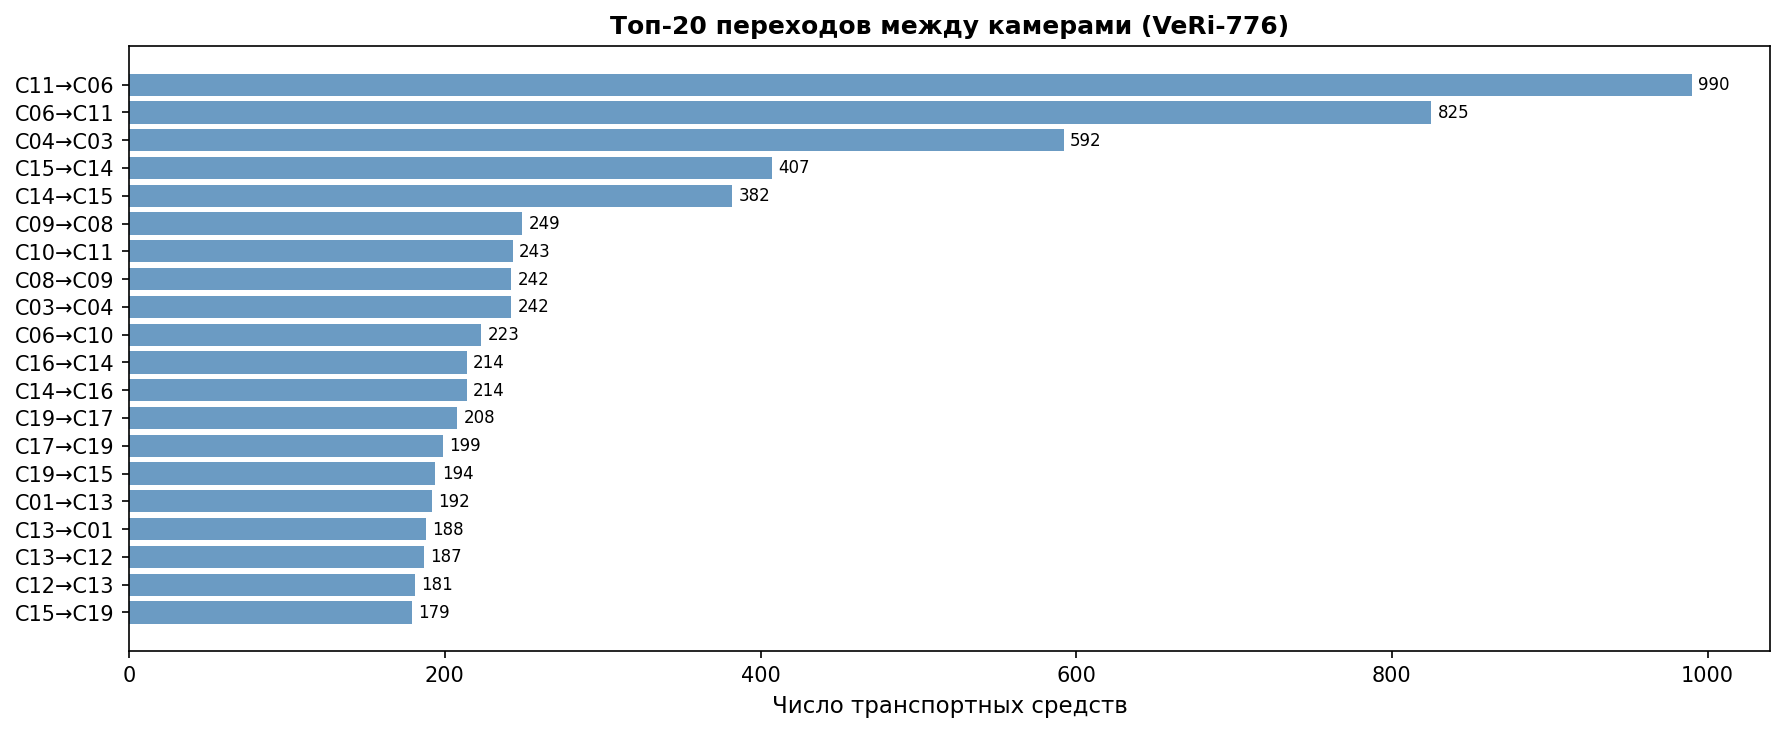
\includegraphics[width=0.85\textwidth]{images/camera_transitions_top20.png}
  \caption{Топ-20 наиболее частых переходов между камерами в обучающей выборке VeRi-776.}
  \label{fig:camera_transitions_top20}
\end{figure}

\subsection{Влияние структуры маршрутов на задачу ReID}

Полученная топология имеет непосредственное значение для оценки качества модели:
протокол \emph{no-same-camera} запрещает сопоставление изображений одной и той же
камеры, поэтому система обязана находить совпадения именно через рёбра данного
графа. Чем длиннее маршрут ТС и чем дальше разнесены камеры, тем сильнее
изменяется внешний вид автомобиля (освещение, ракурс, частичные перекрытия).
Это объясняет, почему трансформерная архитектура ViT-Small, способная строить
глобальные зависимости между частями изображения, превосходит ResNet-50 в условиях
существенных изменений ракурса между камерами.

\section{Анализ кластерной структуры пространства эмбеддингов}
\label{sec:cluster_analysis}

Качество модели повторной идентификации определяется не только финальными метриками
(Rank-1, mAP), но и геометрией пространства эмбеддингов: хорошая модель формирует
компактные внутриклассовые кластеры (малая дисперсия) при большом расстоянии между
кластерами разных идентичностей. Для количественной оценки этого свойства были
извлечены L2-нормированные эмбеддинги обеих моделей на множестве запросов (1\,678
изображений, 200 транспортных средств, 20 камер).

\subsection{PCA-визуализация кластеров по идентичностям}

На рисунках~\ref{fig:pca_resnet} и~\ref{fig:pca_vit} показаны двумерные PCA-проекции
эмбеддингов для 20 наиболее представленных транспортных средств. Звёздочкой отмечен
центроид каждого кластера.

\begin{figure}[H]
  \centering
  \begin{minipage}[t]{0.48\textwidth}
    \centering
    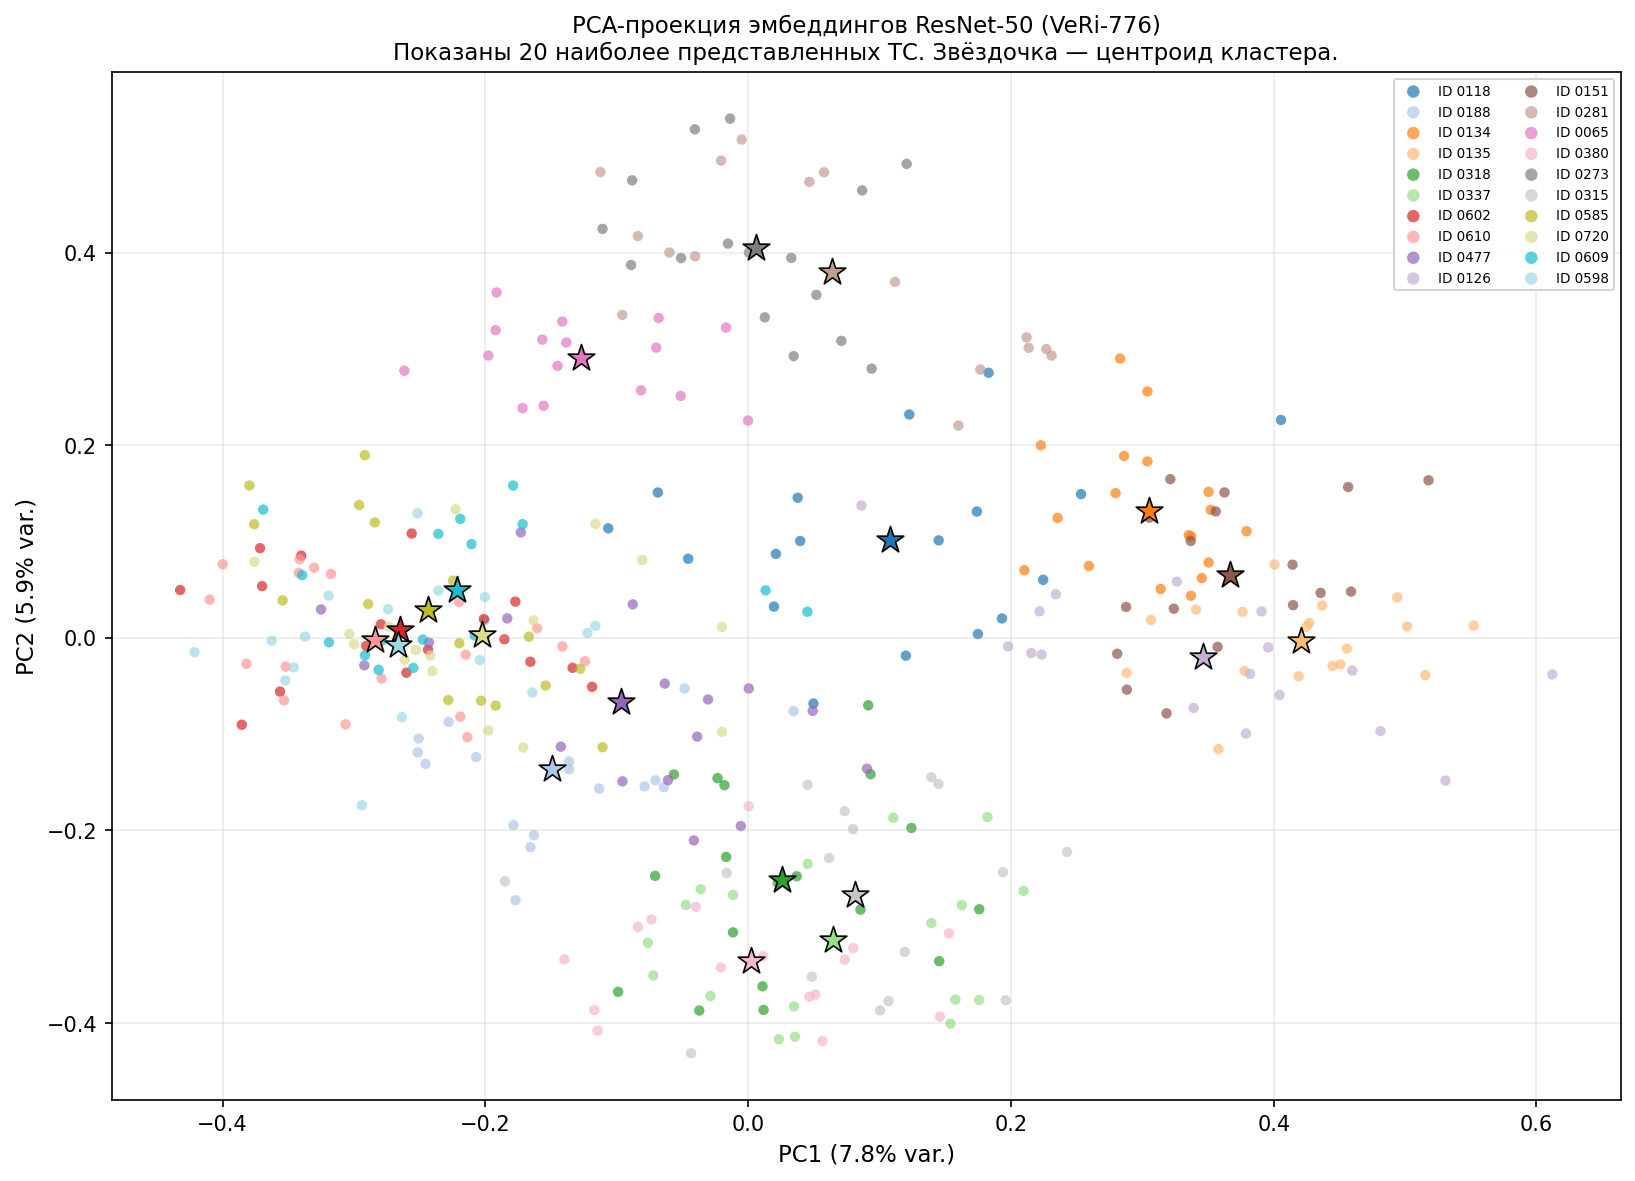
\includegraphics[width=\textwidth]{images/pca_clusters_resnet50.png}
    \caption{PCA-проекция эмбеддингов ResNet-50. Кластеры размыты, значительное
      перекрытие между идентичностями.}
    \label{fig:pca_resnet}
  \end{minipage}
  \hfill
  \begin{minipage}[t]{0.48\textwidth}
    \centering
    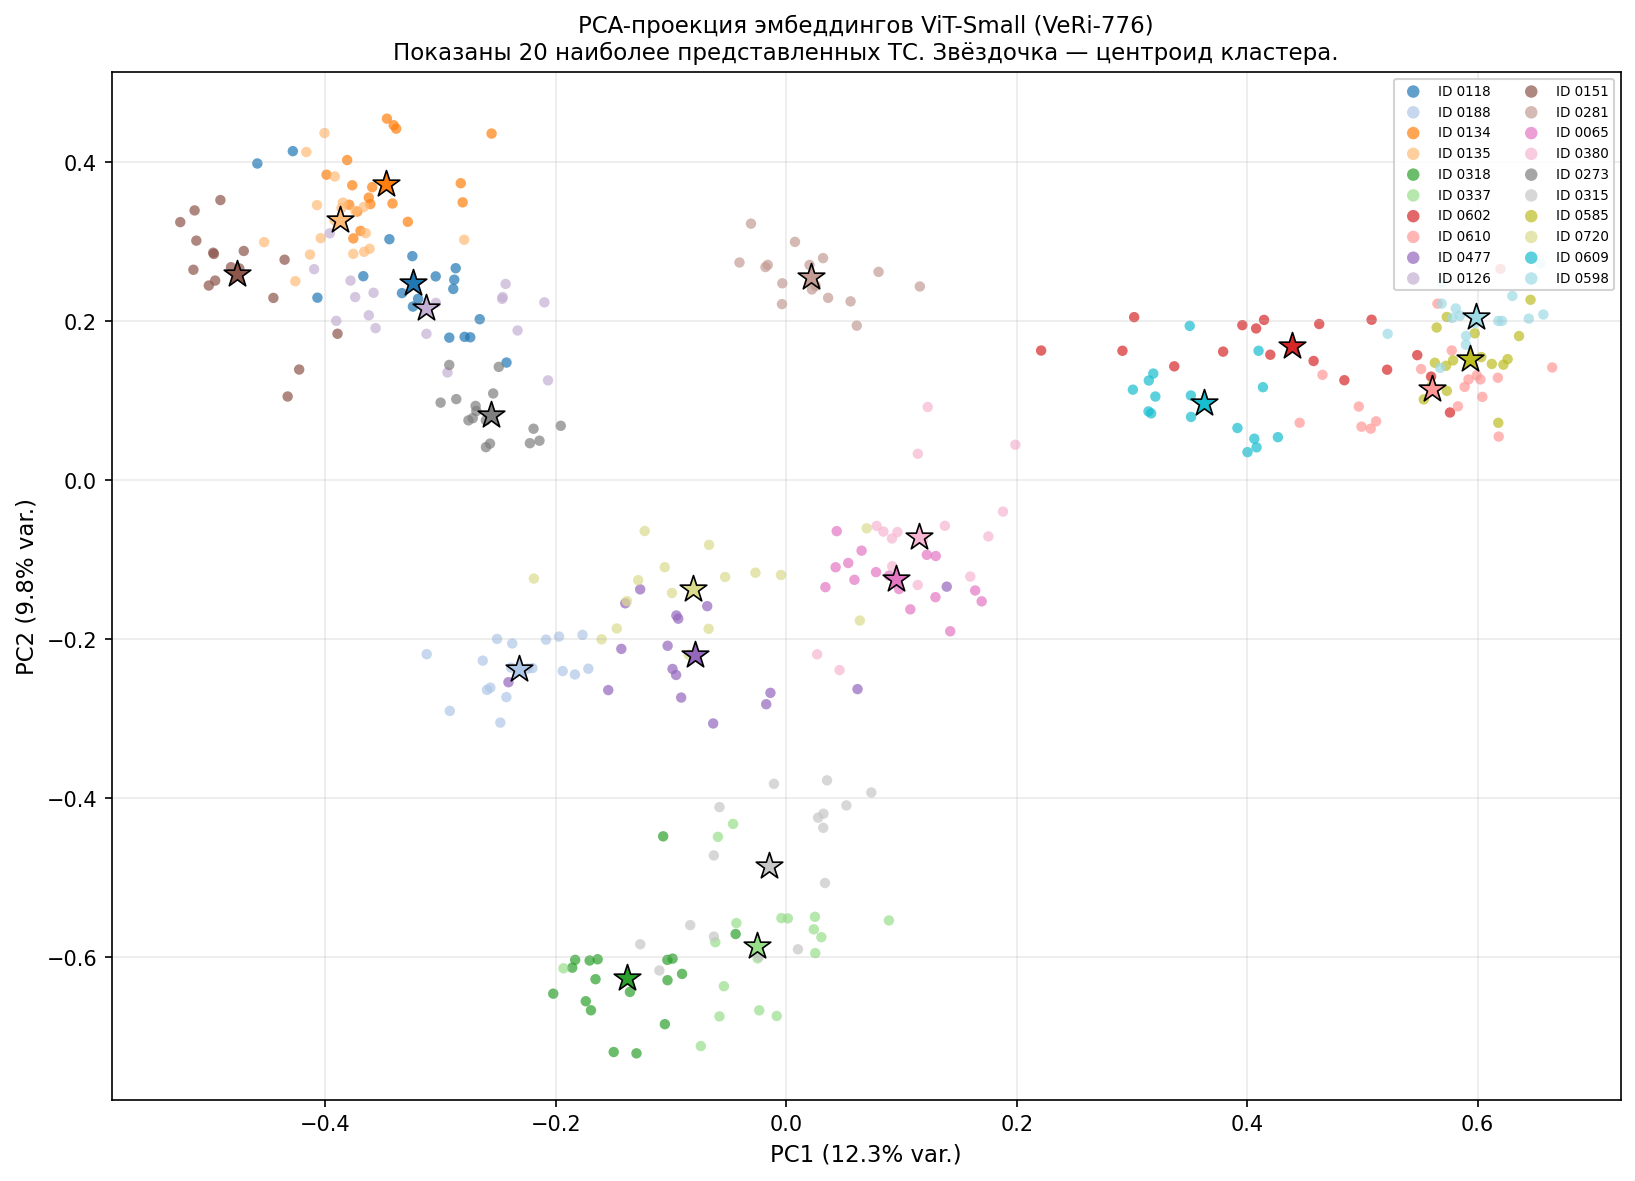
\includegraphics[width=\textwidth]{images/pca_clusters_vit.png}
    \caption{PCA-проекция эмбеддингов ViT-Small. Кластеры заметно компактнее,
      межкластерные расстояния больше.}
    \label{fig:pca_vit}
  \end{minipage}
\end{figure}

\subsection{Количественные метрики компактности}

Для каждой идентичности вычислялась \emph{внутриклассовая дисперсия}~--- среднее
квадратичное L2-расстояние от векторов до центроида класса. Также вычислялись:
среднее расстояние между центроидами разных классов и коэффициент силуэта
(Silhouette score, принимает значения от $-1$ до $+1$, чем выше~--- тем лучше).

\begin{table}[H]
  \centering
  \caption{Метрики кластерной компактности эмбеддингов (запросная выборка VeRi-776)}
  \label{tab:cluster_metrics}
  \begin{tabular}{lcc}
    \hline
    \textbf{Метрика} & \textbf{ResNet-50} & \textbf{ViT-Small} \\
    \hline
    Внутрикл.\ дисперсия (среднее) & 0.4343 & \textbf{0.2471} \\
    Внутрикл.\ дисперсия (медиана) & 0.4394 & \textbf{0.2449} \\
    Межкластерное расстояние       & 0.7872 & \textbf{1.2120} \\
    Коэффициент силуэта            & 0.0240 & \textbf{0.2602} \\
    Отношение межкл./внутрикл.     & 1.19   & \textbf{2.44}   \\
    \hline
  \end{tabular}
\end{table}

\begin{figure}[H]
  \centering
  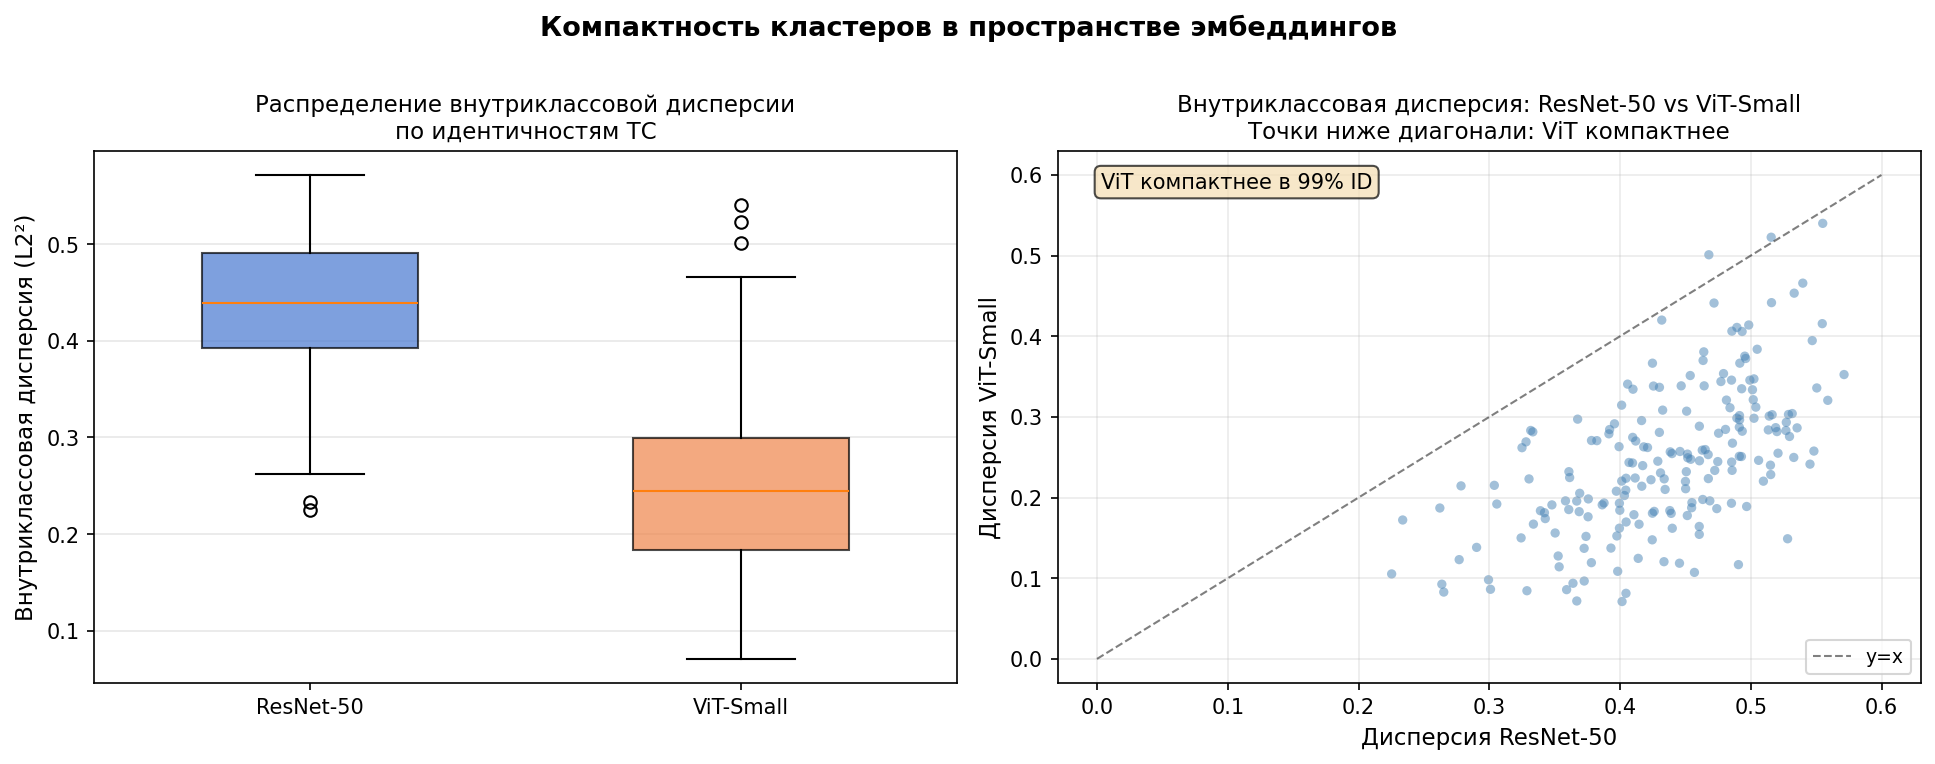
\includegraphics[width=0.92\textwidth]{images/cluster_compactness.png}
  \caption{Слева: распределение внутриклассовой дисперсии по идентичностям ТС.
    Справа: поточечное сравнение дисперсий — точки ниже диагонали означают,
    что ViT-Small формирует более компактный кластер для данного ТС.}
  \label{fig:cluster_compactness}
\end{figure}

Результаты показывают, что ViT-Small формирует значительно более структурированное
пространство эмбеддингов по сравнению с ResNet-50:

\begin{itemize}
  \item внутриклассовая дисперсия ViT-Small в 1.76 раза меньше
    ($0.247$ против $0.434$), что означает более согласованное представление
    одного и того же транспортного средства с разных камер;
  \item межкластерное расстояние у ViT-Small в 1.54 раза больше ($1.212$ против
    $0.787$), то есть разные транспортные средства лучше разделены в пространстве;
  \item коэффициент силуэта ViT-Small ($0.260$) более чем в 10 раз превышает
    аналогичный показатель ResNet-50 ($0.024$), что подтверждает существенно
    более чёткую кластерную структуру;
  \item отношение межкластерного расстояния к среднеквадратичному радиусу
    внутриклассового кластера составляет $2.44$ для ViT-Small против $1.19$
    для ResNet-50 — улучшение в 2 раза.
\end{itemize}

Данные результаты согласуются с известным свойством механизма
само-вни\-ма\-ния~(self"=at\-ten\-tion): глобальный контекст позволяет модели игнорировать
локальные изменения (ракурс, освещение, частичные перекрытия) и концентрироваться
на дискриминативных признаках кузова и формы автомобиля.

\section{Анализ качества идентификации по парам камер}
\label{sec:camera_heatmap}

Совокупные метрики (Rank-1, mAP) усредняют качество по всем парам запрос–галерея.
Для более детального понимания ошибок модели проведён пространственный анализ:
для каждой пары $(C_q, C_g)$ — камера запроса и камера галереи — вычислена
точность Rank-1 при поиске только среди изображений камеры $C_g$.

\subsection{Тепловые карты Rank-1 по парам камер}

\begin{figure}[H]
  \centering
  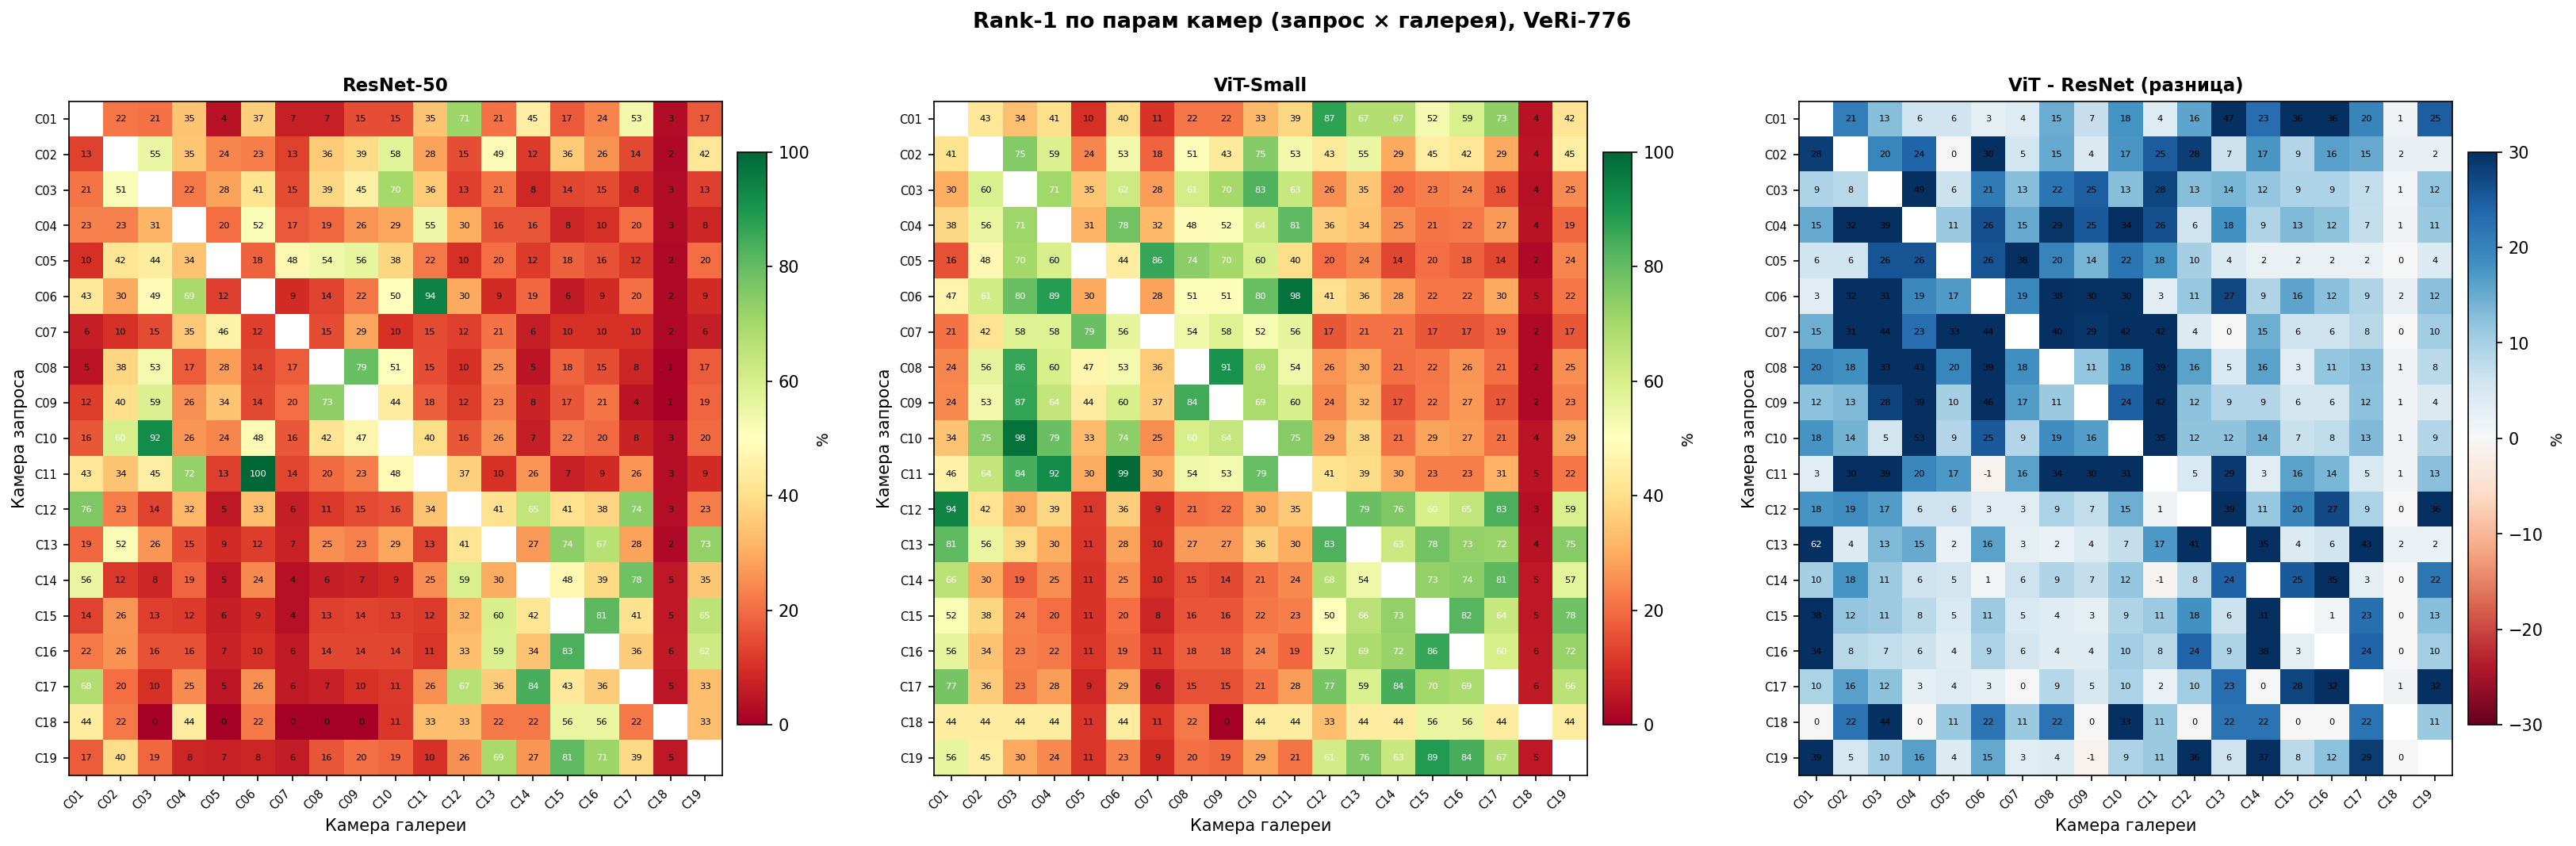
\includegraphics[width=\textwidth]{images/camera_heatmap_comparison.png}
  \caption{Rank-1~(\%) по парам камер запроса и галереи. Слева~--- ResNet-50,
    в центре~--- ViT-Small, справа~--- разность (зелёный: ViT лучше,
    красный: ResNet лучше). Диагональ пуста~--- протокол \emph{no-same-camera}.}
  \label{fig:camera_heatmap}
\end{figure}

Тепловые карты демонстрируют ярко выраженную неоднородность качества:

\begin{itemize}
  \item \textbf{Лучшие пары}: переход $\mathrm{C11} \to \mathrm{C06}$ даёт
    Rank-1~$= 100\%$ (ResNet-50) и $98.9\%$ (ViT-Small) — камеры расположены
    близко, условия съёмки схожи;
  \item \textbf{Проблемная камера~C18}: все пары с участием камеры~18 показывают
    низкий Rank-1 ($0$--$2.3\%$), что свидетельствует о кардинально иных условиях
    съёмки (возможно, иной ракурс, освещение или высота монтажа);
  \item ViT-Small превосходит ResNet-50 на \textbf{322 из 342} ненулевых пар
    ($94.2\%$ пар), средний Rank-1: $41.3\%$ против $26.2\%$ (+57.6\%
    относительное улучшение).
\end{itemize}

\begin{table}[H]
  \centering
  \caption{Топ-5 наиболее лёгких и сложных пар камер по Rank-1}
  \label{tab:camera_pairs}
  \begin{tabular}{llcc}
    \hline
    \textbf{Тип} & \textbf{Пара} & \textbf{ResNet-50} & \textbf{ViT-Small} \\
    \hline
    \multirow{5}{*}{Лёгкие} &
      C11 $\to$ C06 & 100.0\% & 98.9\% \\
    & C06 $\to$ C11 & 94.3\%  & 97.7\% \\
    & C10 $\to$ C03 & 92.3\%  & 97.8\% \\
    & C17 $\to$ C14 & 83.8\%  & — \\
    & C16 $\to$ C15 & 83.3\%  & — \\
    \hline
    \multirow{3}{*}{Сложные} &
      C18 $\to$ C03 & 0.0\%  & — \\
    & C18 $\to$ C05 & 0.0\%  & — \\
    & C18 $\to$ C07 & 0.0\%  & 2.1\% \\
    & C18 $\to$ C08 & 0.0\%  & 2.3\% \\
    & C18 $\to$ C09 & 0.0\%  & 0.0\% \\
    \hline
  \end{tabular}
\end{table}

Полученный результат подчёркивает практическую ценность пространственного анализа:
проблемная камера~C18 не была бы выявлена при анализе только суммарных метрик.
В реальной системе видеонаблюдения это указывало бы на необходимость технического
обслуживания или перенастройки данной камеры.

\section{Реидентификация в связке с детектором YOLOv11}
\label{sec:yolo_reid}

\subsection{Демонстрация пайплайна}

На рисунке~\ref{fig:yolo_reid_demo} показан результат работы полного пайплайна:
YOLOv11n детектирует транспортное средство на входном изображении (красная рамка),
после чего ViT-Small выполняет реидентификацию в галерее.
Для каждого запроса отображаются три ближайших кандидата из тестовой галереи
с косинусным расстоянием.

\begin{figure}[H]
  \centering
  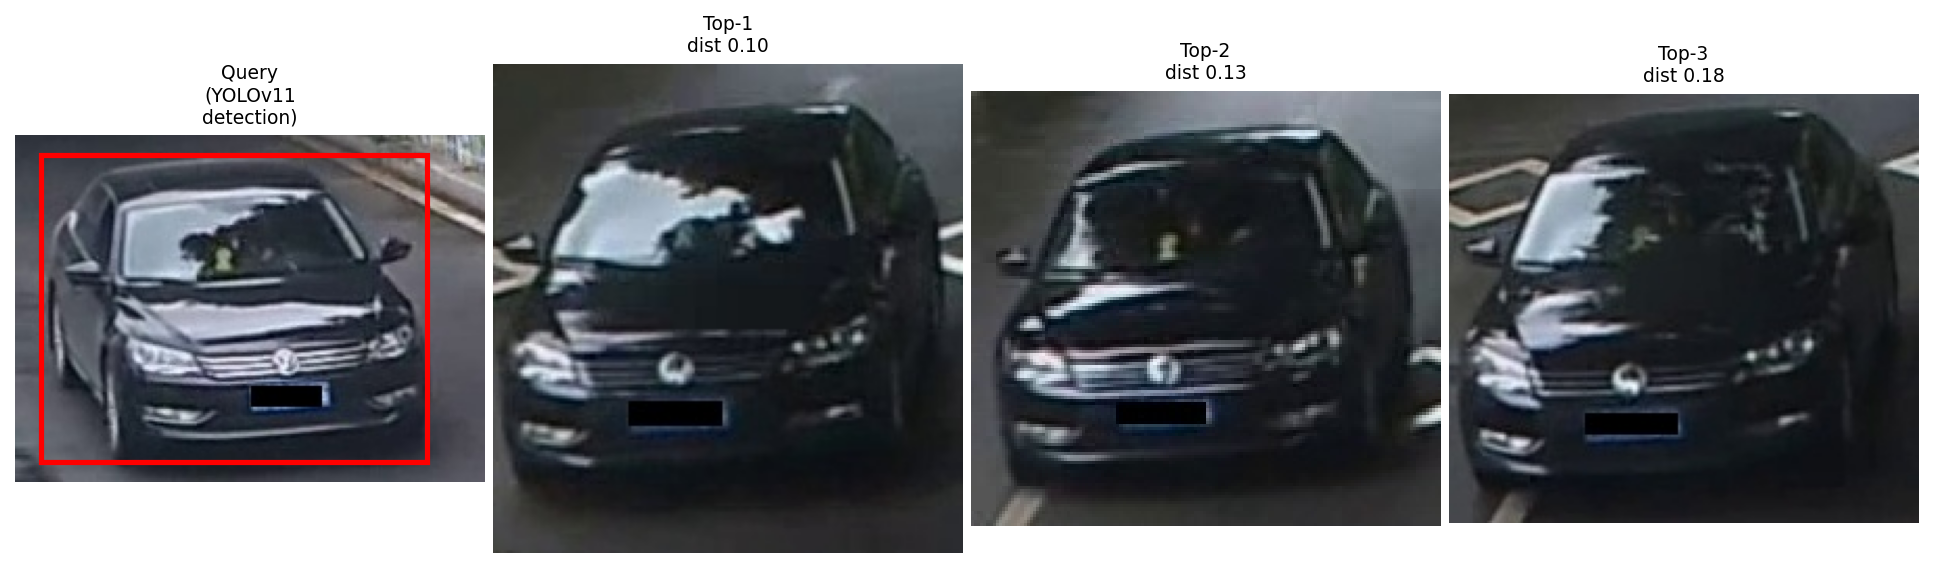
\includegraphics[width=0.95\textwidth]{images/yolo_reid_demo.png}
  \caption{Пример работы пайплайна YOLOv11 + ViT-Small: запрос с bbox (крайний
    левый столбец) и топ-3 результата поиска по галерее; косинусное расстояние указано над каждым изображением.}
  \label{fig:yolo_reid_demo}
\end{figure}

\subsection{Влияние качества детекции на метрики}

Датасет VeRi-776 содержит заранее вырезанные изображения транспортных средств
(GT-кропы). Для оценки влияния детектора на качество реидентификации проведён
следующий эксперимент: вместо GT-кропа запроса в модель подаётся crop, полученный
YOLOv11n из того же изображения. Это моделирует реальный сценарий, в котором bbox
поступает от детектора, а не из ручной разметки.
Эмбеддинги галереи при этом остаются прежними (GT-кропы).

\begin{table}[H]
\centering
\caption{Сравнение ReID с GT-кропом и YOLO-кропом запроса (ViT-Small, VeRi-776)}
\label{tab:yolo_vs_gt}
\begin{tabular}{lcccc}
\hline
\textbf{Метод запроса} & \textbf{Rank-1} & \textbf{Rank-5} & \textbf{mAP} & \textbf{Fallback} \\
\hline
ViT-Small (GT crop)   & 90.05\% & 96.25\% & 69.41\% & --- \\
ViT-Small (YOLO crop) & 85.88\% & 91.95\% & 65.54\% & 21.5\% \\
\hline
\end{tabular}
\end{table}

Разница метрик между GT-кропом и YOLO-кропом характеризует чувствительность
модели ReID к точности локализации детектора: если метрики близки,
система устойчива к шуму детектора; значительный провал указывает на
необходимость улучшения этапа детекции.

\section{Анализ расстояния Махаланобиса}

Расстояние Махаланобиса учитывает корреляционную структуру признакового пространства:
\[
  d_M(x, y) = \sqrt{(x - y)^\top \Sigma^{-1} (x - y)},
\]
где $\Sigma$ --- ковариационная матрица, оцениваемая по тренировочным эмбеддингам.
Цель --- проверить, улучшает ли перераспределение пространства эмбеддингов качество поиска.

\subsection{Постановка эксперимента}

Ковариационная матрица оценивается по 5\,000 случайно выбранных тренировочных
эмбеддингов с гребневой регуляризацией ($\varepsilon = 10^{-5}$).
Для ResNet-50 ($D=2048$) используется диагональное приближение ковариации
(вычислительное ограничение); для ViT-Small ($D=384$) --- полная матрица.

\subsection{Результаты}

\begin{table}[H]
\centering
\caption{Сравнение L2 и расстояния Махаланобиса на VeRi-776}
\label{tab:mahalanobis}
\begin{tabular}{l|l|c|c|c}
\hline
\textbf{Модель} & \textbf{Метрика} & \textbf{L2} & \textbf{Махаланобис} & \textbf{$\Delta$} \\
\hline
ResNet-50 & Rank-1 & 88.68 & 88.74 & $+0.06$ \\
          & Rank-5 & 94.64 & 94.76 & $+0.12$ \\
          & mAP    & 64.27 & 64.55 & $+0.28$ \\
\hline
ViT-Small & Rank-1 & 90.05 & 83.43 & $-6.62$ \\
          & Rank-5 & 96.25 & 90.52 & $-5.72$ \\
          & mAP    & 69.41 & 38.43 & $-30.98$ \\
\hline
\end{tabular}
\end{table}

\subsection{Анализ результатов}

Для ResNet-50 диагональное приближение Махаланобиса эквивалентно нормировке
признаков на стандартное отклонение и практически не отличается от L2 ($\Delta$mAP~$+0.28\%$).

Для ViT-Small полная матрица Махаланобиса \emph{ухудшает} все метрики
(mAP падает на $31\%$). Причина: ReID-эмбеддинги подвергаются L2-нормализации
перед поиском и лежат на единичной гиперсфере~$\mathcal{S}^{383}$.
На гиперсфере косинусное (= L2 для нормированных векторов) расстояние геометрически
корректно, тогда как Махаланобис в евклидовом пространстве нарушает эту структуру:
оценённая ковариация описывает облако, а не сферу, что приводит к деградации ранжирования.

\textbf{Вывод:} для нормированных гиперсферических эмбеддингов косинусное расстояние
является оптимальным выбором; замена на Махаланобис не даёт выигрыша и может привести
к существенной деградации качества поиска.

\section{Визуализация карт внимания ViT-Small}

Механизм self-attention является ключевым преимуществом трансформерной архитектуры.
Для интерпретации работы модели были визуализированы карты внимания (attention maps)
ViT-Small~--- внимание CLS-токена к пространственным патчам изображения,
агрегированное по последним четырём трансформерным блокам с операцией максимума
по головам~\cite{dosovitskiy2020image}.

\subsection{Метод извлечения карт внимания}

Классический метод Attention Rollout~\cite{abnar2020quantifying},
перемножающий усреднённые по головам матрицы внимания всех $L=12$ блоков,
для дообученного на ReID ViT даёт практически равномерные карты:
произведение большого числа сглаженных матриц быстро сходится к равномерному
распределению, и дискриминативный сигнал теряется. Поэтому в работе применяется
агрегация внимания только из \emph{последних} $K=4$ блоков с операцией максимума
по головам, что сохраняет сигнал наиболее «сфокусированных» голов.

Пусть $\mathbf{A}_l^{(h)} \in \mathbb{R}^{N \times N}$~--- матрица внимания
головы $h$ блока $l$ ($N = 197$ токенов, $H = 6$ голов). Строка CLS-токена
к патч-токенам в блоке $l$:
\[
  \mathbf{a}_l^{(h)} = \mathbf{A}_l^{(h)}[0,\,1{:}] \;\in\; \mathbb{R}^{196}.
\]
По каждому из последних $K = 4$ блоков ($l = L-3, \dots, L$) вычисляется
максимум по головам и затем среднее по этим слоям:
\[
  \mathbf{m}_l = \max_{h=1,\dots,H} \mathbf{a}_l^{(h)},
  \qquad
  \mathbf{m} = \frac{1}{K}\sum_{l=L-K+1}^{L} \mathbf{m}_l \;\in\; \mathbb{R}^{196}.
\]
Полученный вектор $\mathbf{m}$ преобразуется в решётку $14 \times 14$ и
масштабируется до размера исходного изображения билинейной интерполяцией.
Перед наложением применяется перцентильная нормализация: значения отсекаются
по $5$-му и $95$-му перцентилям и линейно растягиваются в $[0,1]$~--- это
предотвращает «выжигание» карты единичными выбросами. Тепловая карта
накладывается на изображение с коэффициентом смешивания $\alpha = 0.55$
и цветовой схемой \emph{jet}.

\subsection{Примеры карт внимания}

\begin{figure}[H]
  \centering
  \includegraphics[width=0.5\textwidth]{images/attention_maps_vit}
  \caption{Карты внимания ViT-Small для случайных запросов из VeRi-776.
           Модель концентрирует внимание преимущественно на форме кузова
           и характерных деталях (надписи, элементы кузова); на сложных
           ракурсах (вид сверху, частичное перекрытие) внимание частично
           рассеивается на фоновые области.}
  \label{fig:attention_maps}
\end{figure}

\subsection{Успешные и ошибочные совпадения}

\begin{figure}[H]
  \centering
  \includegraphics[width=0.72\textwidth]{images/attention_success_fail_vit}
  \caption{Карты внимания ViT-Small при верных (зелёная рамка) и ошибочных
           (красная рамка) совпадениях Rank-1.
           При успешном поиске модель фокусируется на уникальных деталях:
           государственный номер, рисунок диска, спойлер.
           При ошибке~--- на общей форме и цвете, что приводит к смешению
           схожих транспортных средств.}
  \label{fig:attention_success_fail}
\end{figure}

\subsection{Выводы по картам внимания}

Анализ attention maps подтверждает, что ViT-Small обучился выделять
семантически значимые области изображения без явной разметки частей автомобиля:
\begin{itemize}
  \item при верных совпадениях: фокус на дискриминативных деталях (номер, диски, уникальные элементы кузова);
  \item при ошибках: размытое внимание на форме и цвете, что типично для сложных случаев с визуально схожими автомобилями;
  \item в отличие от CNN (GradCAM), ViT обеспечивает глобальный контекст уже в первых блоках, что объясняет устойчивость к частичному перекрытию.
\end{itemize}

\section{Обсуждение результатов}

\subsection{Сравнительный анализ CNN vs Transformer}

На основе проведённых экспериментов:

\begin{itemize}
  \item \textbf{Качество:} ViT-Small показывает лучшие результаты из всех трёх моделей: Rank-1 90.0\%, mAP 69.4\%. ResNet-101 уступает даже ResNet-50 (Rank-1 86.7\%, mAP 57.7\%), что демонстрирует: глубина CNN без изменения архитектурной парадигмы не решает задачу лучше. Механизм self-attention трансформера эффективнее для Vehicle ReID.
  \item \textbf{Сходимость:} ViT требует меньше эпох (50 vs 120), но больший warmup (10 vs 5 эпох) из-за чувствительности к начальному learning rate.
  \item \textbf{Размер модели:} ViT-Small (21.9M параметров) компактнее ResNet-50 (24.7M) и тем более ResNet-101 (43.7M), при этом показывает наилучшее качество.
\end{itemize}

\subsection{Ключевые выводы}
\begin{enumerate}
  \item BNNeck + Triplet Loss — ключевые компоненты для метрического обучения;
  \item Аугментации (Random Erasing, ColorJitter) повышают робастность;
  \item ViT-Small превосходит ResNet-50 по качеству (+5.1\% mAP) благодаря глобальному вниманию.
\end{enumerate}

\textbf{Ограничения:} эксперименты на статичных кропах; для сильного domain shift может потребоваться domain adaptation.

